
\chapter{Обсуждение Результатов}\label{chapt_results}
В результате полугода работы прибора ДЭПРОН накоплен большой массив информации - 35 тысяч файлов бинарных данных, общим объемом 141 МБайт. Эти данные являются сжатыми и после распаковки в человеко-читаемый табличный вид представлены массивом файлов объемом 1,3 Гб, эти данные собраны в файлы по дням года и осуществлена привязка данных к географическим и геомагнитным координатам.



Далее информация прибора ДЭПРОН была визуализирована с помошью пакета \texttt{lattice} и базовой графической системы R. На рисунке \ref{fig:depronseclog08-29-16} показаны результаты визуализации.
\begin{figure}[h]
	\centering
	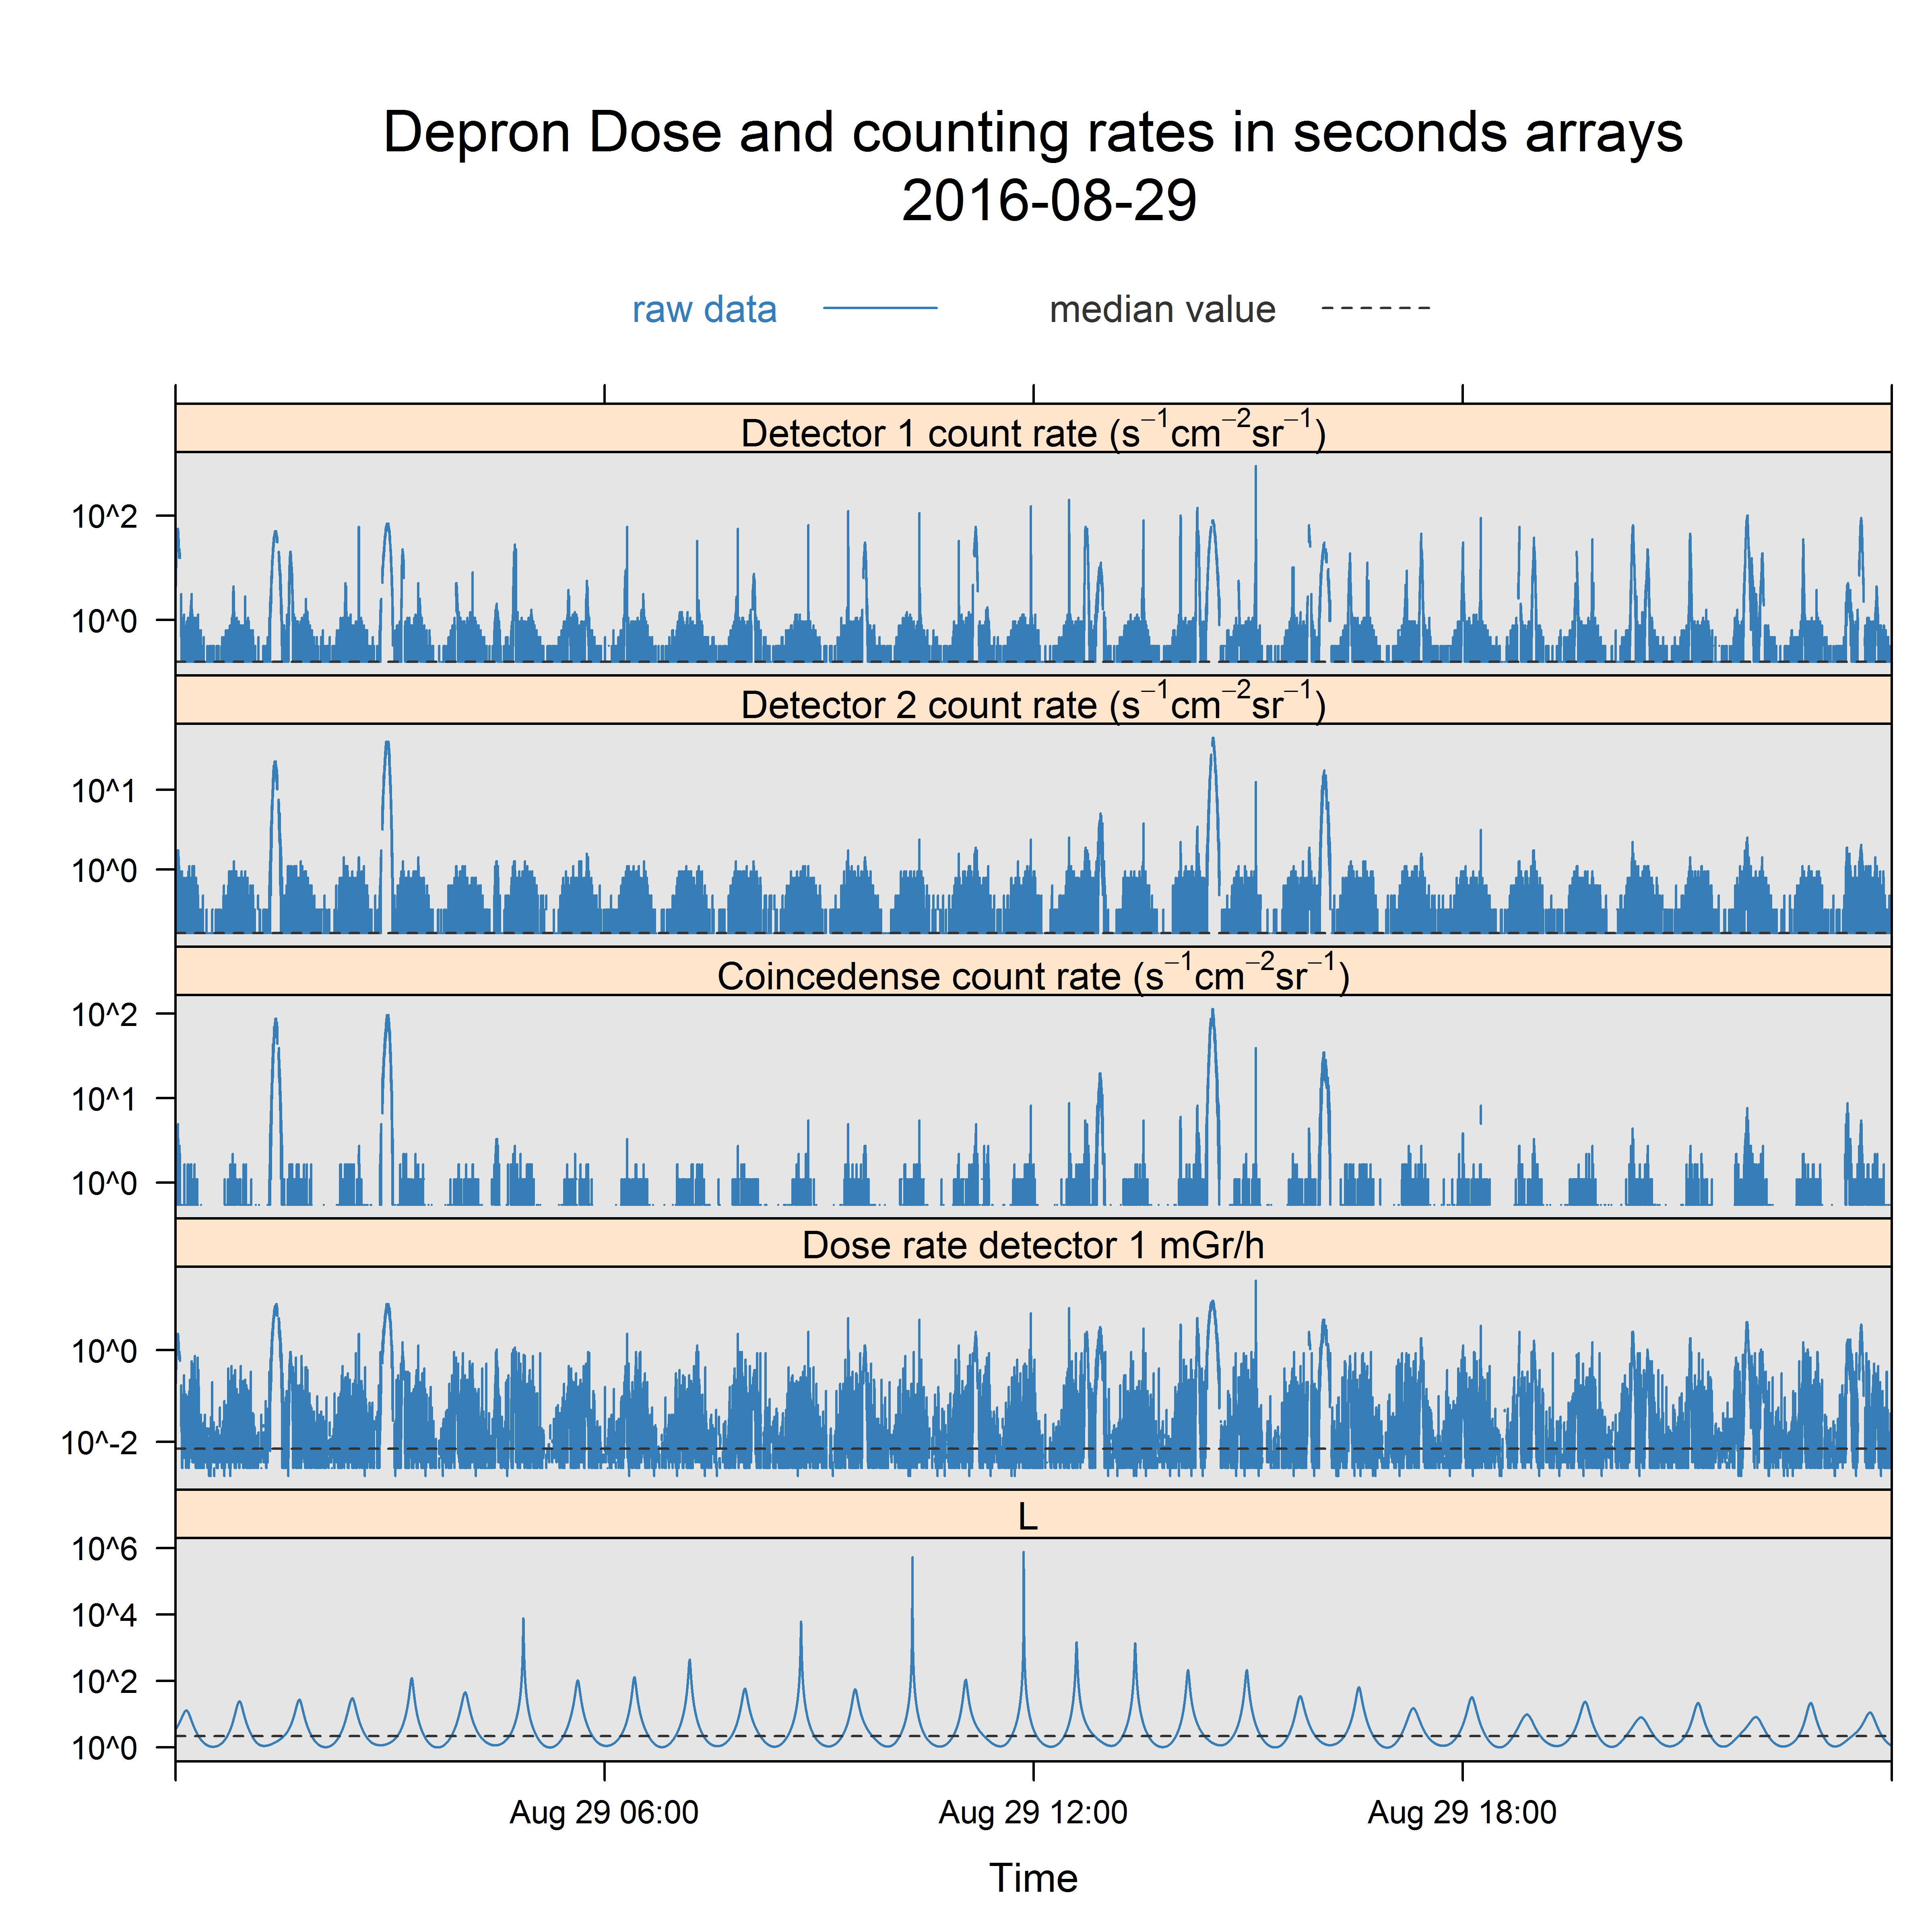
\includegraphics[width=0.5\linewidth]{images/results/depron_sec_log08-29-16}
	\caption{Временные серии  измерений детекторов прибора ДЭПРОН. }
	\label{fig:depronseclog08-29-16}
\end{figure}
Так как секундные данные содержат существенный разброс значений из-за малой статистики отсчетов, был предложен и реализован алгоритм треугольного сглаживания, который позволяет выявлять только значимые изменения в исходных данных. Пример использования этого алгоритма показан на рисунке 	\ref{fig:depronseclognew08-29-16}.
\begin{figure}
	\centering
	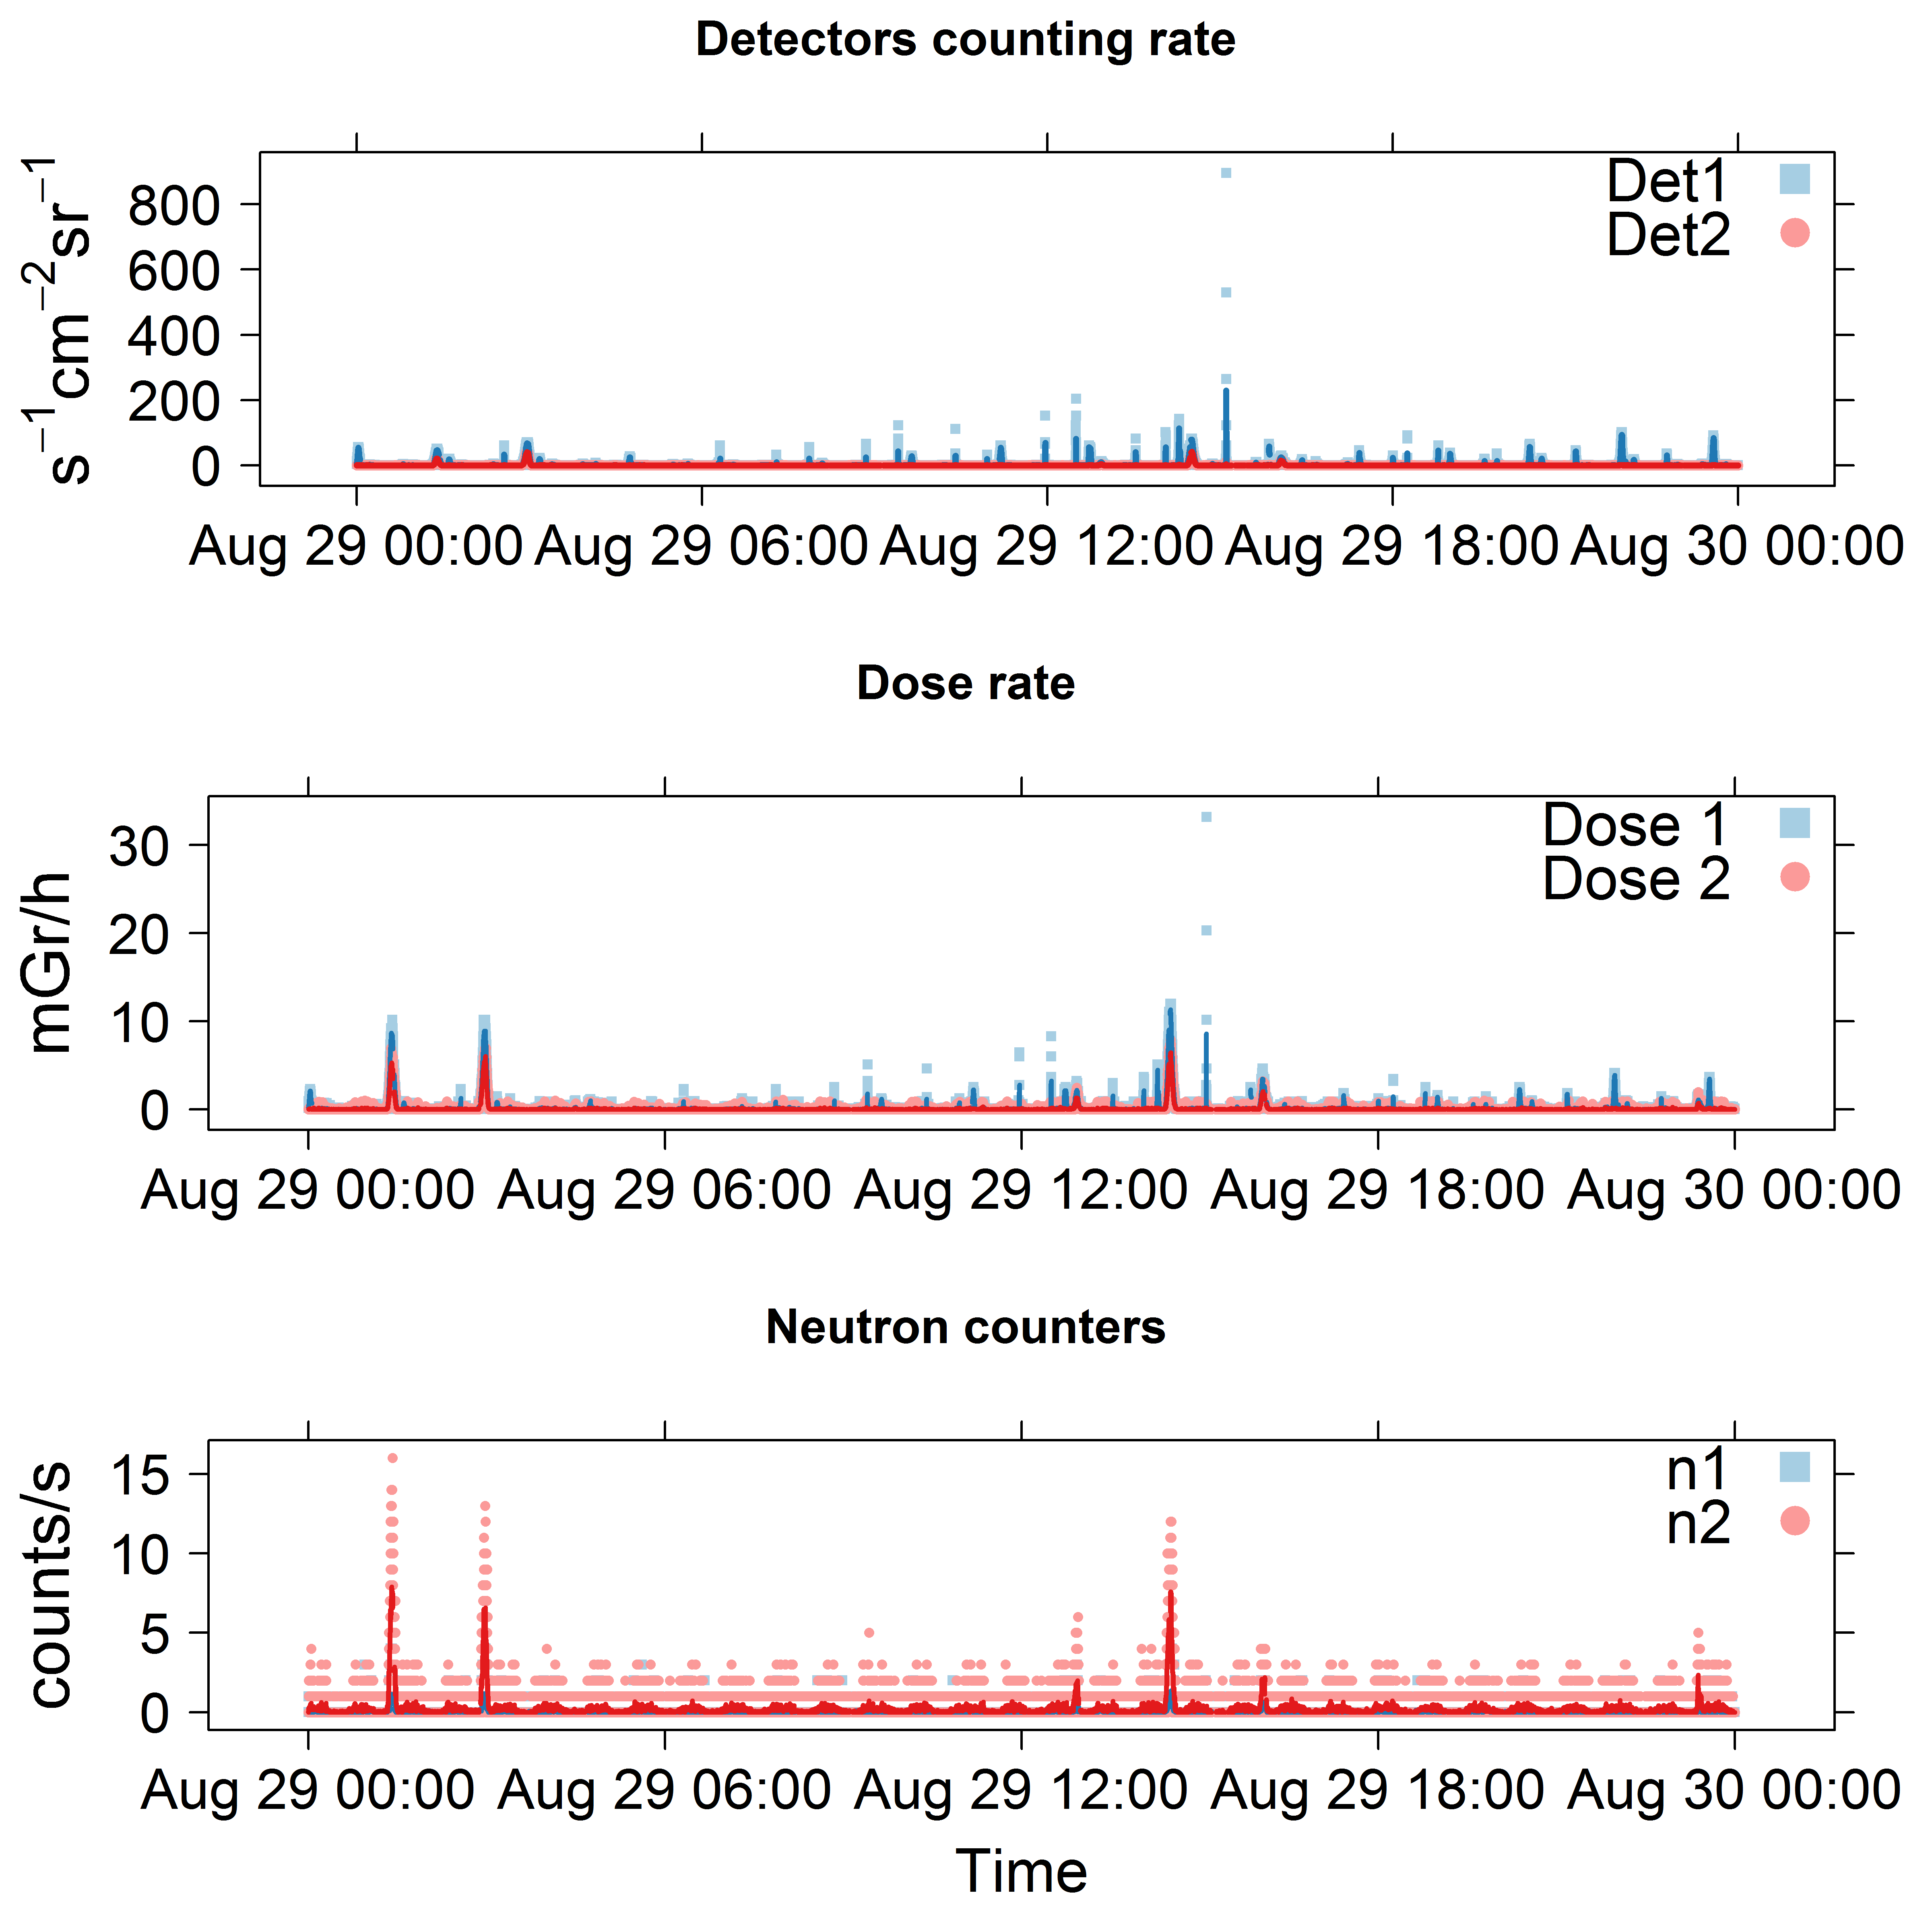
\includegraphics[width=0.5\linewidth]{images/results/depron_sec_log_new08-29-16}
	\caption{Временные серии измерений ДЭПРОН со сглаживанием. }
	\label{fig:depronseclognew08-29-16}
\end{figure}
В первую очередь для каждого дня работы прибора были построены карты скоростей счета в первом детекторе \ref{sec:planetDose}.В процессе построения пространственного распределения было обнаружено расхождение меток времени  ДЭПРОН и всемирного времени. Разработанное решение проблемы привязки данных подробно рассматривается в разделе \ref{sec3.2}.

Аналогично картам, были построены долготные зависимости скоростей счета в первом детекторе, эти графики позволили оперативно заметить резкие всплески потоков частиц во внешнем радиационном поясе \label{sec:flash_analisys}. Также для каждого дня были построены карты скоростей счета в координатах Мак-Илвайна \cite{McIlwain1961}, которые были рассчитанны по модели IGRF.

\section{Планетарное распределение потоков частиц, мощности дозы на высоте полета КА а также потоков нейтронов} \label{sec:planetDose}
При последующей обработке данных были построены графики географического распределения скоростей счета во всех детекторах прибора - двух полупроводниковых и двух нейтронных счетчиков. Цветовая схема для карт подобрана таким образом, чтобы максимальные значения были отображены красным цветом а минимальные синим, между конечными точками цвет изменяется по градиенту. Цветовая палитра квантована на 20 дискретных цветов. Каждому значению полученной дозы ставится в соответствие индекс в массиве цветов, который вычисляется по формуле:
\begin{equation*}
index_{color} = \begin{cases}
	8*\log{10}(N + 1)+1,  & \text{если } 8*\log{10}(N + 1) +1 < n \\
	n,  & \text{если } 8*\log{10}(N + 1) +1 \ge n
	\end{cases}
\end{equation*}
		где $ n $ -- цветность палитры, а $ N $ -- величина, подлежащая отображению.
						
% col = colr[ifelse(ceiling(8*log10(as.integer(combined.zoom$count1)+1))+1>n,
%n,
%ceiling(8*log10(as.integer(combined.zoom$count1)+1))+1)]
%
На картах 	\ref{fig:depronmap241} каждый маркер представляет результаты измерений детекторов за одну секунду. В качестве маркера выбран незакрашенный круг, так как в отличие от точки или линии он позволяет покрыть некоторую площадь на графике. Размер маркера подобран исходя из соображений заметания определенной площади, так как  при полете по орбите спутник покрывает 7,5 км каждую секунду. Маркеры частично перекрываются, особенно в полярных областях и наилучшие результаты по отображению были получены при использовании частичной прозрачности. Для простоты отображения выбрана прямоугольная проекция карты по широте и долготе, поэтому на различных широтах площадь отображаемой поверхности не искажена. Это обстоятельство таким образом лишь условно соотвествует величине траектории вдоль которой производилось измерение.
\begin{figure}[h]
	\centering
	\includegraphics[width=0.7\linewidth]{images/depronmap241}
	\caption{Карта распределения счета в первом детекторе.}
	\label{fig:depronmap241}
\end{figure}

\section{Распределение мощности дозы вне радиационных поясов Земли}
Данные за все время измерений были разделены на зоны соответствующие участкам траектории, проходящим через ЮАА, внешний радиационный пояс, а также всем оставшимся участкам траектории спутника. Разделение было проведено по геомагнитным координатам. 
\begin{verbatim}
combined.zoom.anom<-filter(combined, b<0.21)
combined.zoom.polar <-filter(combined,l<7,l>3)
combined.zoom.regular<-filter(combined,l>7|l<3,b>0.21)
\end{verbatim}
Разделение по геомагнитным координатам позволило для большинства дней отделить высокие по величине вклады ЮАА и авроральных областей, оставшиеся части траектории несут радиационную нагрузку, показанную на рисунке \ref{fig:gcrdose}. 
\begin{figure}
	\centering
	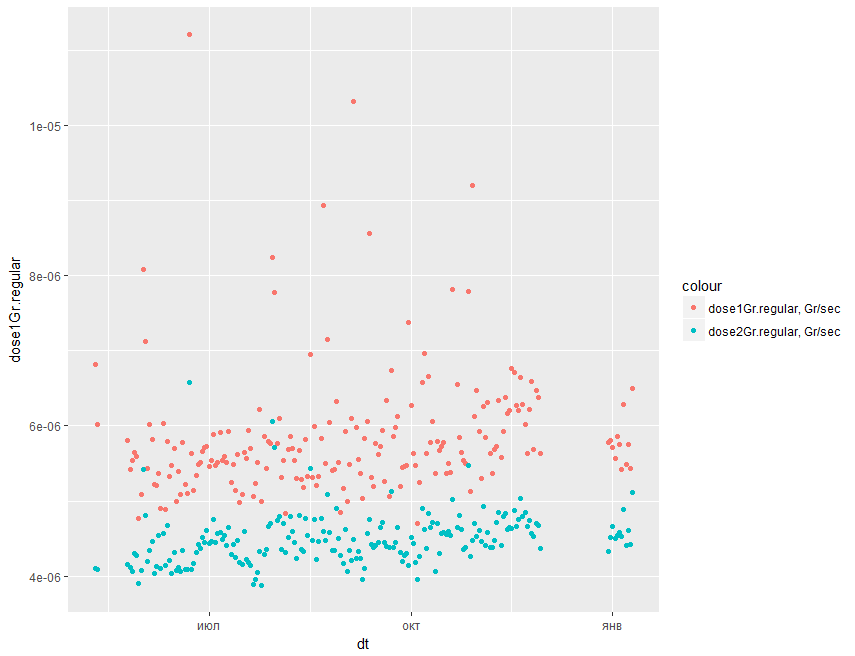
\includegraphics[width=0.5\linewidth]{images/doseanalisys/GCRdose}
	\caption{Поглощенные дозы за сутки, полученные при полете спутника вне ЮАА и внешнего радиационного пояса. Основной вклад в дозу вносит ГКЛ.}
	\label{fig:gcrdose}
\end{figure}
Основной вклад в поглощенную дозу в этих зонах вносит ГКЛ, которое слабо моделируется солнечной активностью и на протяжении годового цикла измерений в 2016 году меняется незначительно, этот факт подтверждается надежными измерениями сети наземных нейтронных мониторов \ref{fig:nmdb2016}. Тем не менее, на выделенных зонах видно несколько выбросов до величин мощности дозы в 10\textsuperscript{-4} Гр/с. Эти выбросы свидетельствуют, что разделение по геомагнитным координатам не позволяет полностью отделять авроральную зону и ЮАА. Причина вероятно заключается в возмущенной геомагнитной обстановке в эти периоды времени, она приводит к смещению реальных значений B и L, относительно расчетных по модели IGRF, которые были использованы при привязке данных ДЭПРОН.

\begin{figure}
	\centering
	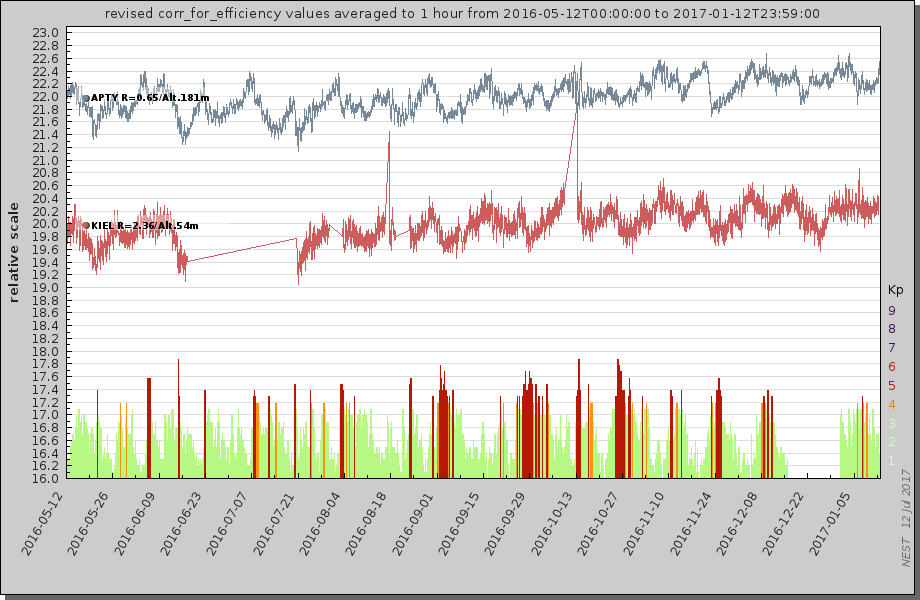
\includegraphics[width=0.7\linewidth]{images/nmdb2016}
	\caption{Данные нейтронным мониторов за период работы прибора ДЭПРОН в 2016-207 гг. По материалам из базы данных \href{www.nmdb.eu}{NMDB}, основанную в рамках программы Европейского союза FP7 (контракт № 213007) для предоставления данных \cite{Ibragimov}. Верхняя кривая представляет данные нейтронного монитора в Апатитах, нижняя кривая представляет данные монитора в Киль, Германия. Измерения представлены в относительных единицах, нормированных на атмосферное давление и эффективность регистрации.}
	\label{fig:nmdb2016}
\end{figure}

\section{Распределения мощности дозы в области ЮАА}
Из результатов исследований НИИЯФ МГУ \cite{Lishnevskii2012} известно, что дозы,  набираемые при пролетах МКС через области аномалии являются значительными несмотря на малые участки траектории пересекающие аномалию. Аналогичная ситуация возникает и на высокоширотной полярной орбите, это подтверждают данные ДЭПРОН, так как он работает на полярном аппарате Ломоносов. 

В качестве примера возьмем временные серии скоростей счета и мощности дозы, полученные с ДЭПРОН для 14:30 29 Августа 2016 года \ref{fig:depronseclognew08-29-1614-24-23}. Возрастание скоростей счета и доз связано с пересечением ЮАА. Точками показаны измерения с детекторов с секундным разрешением, сплошными линиями отражено сглаживание данных треугольным фильтром.

\begin{figure}
	\centering
	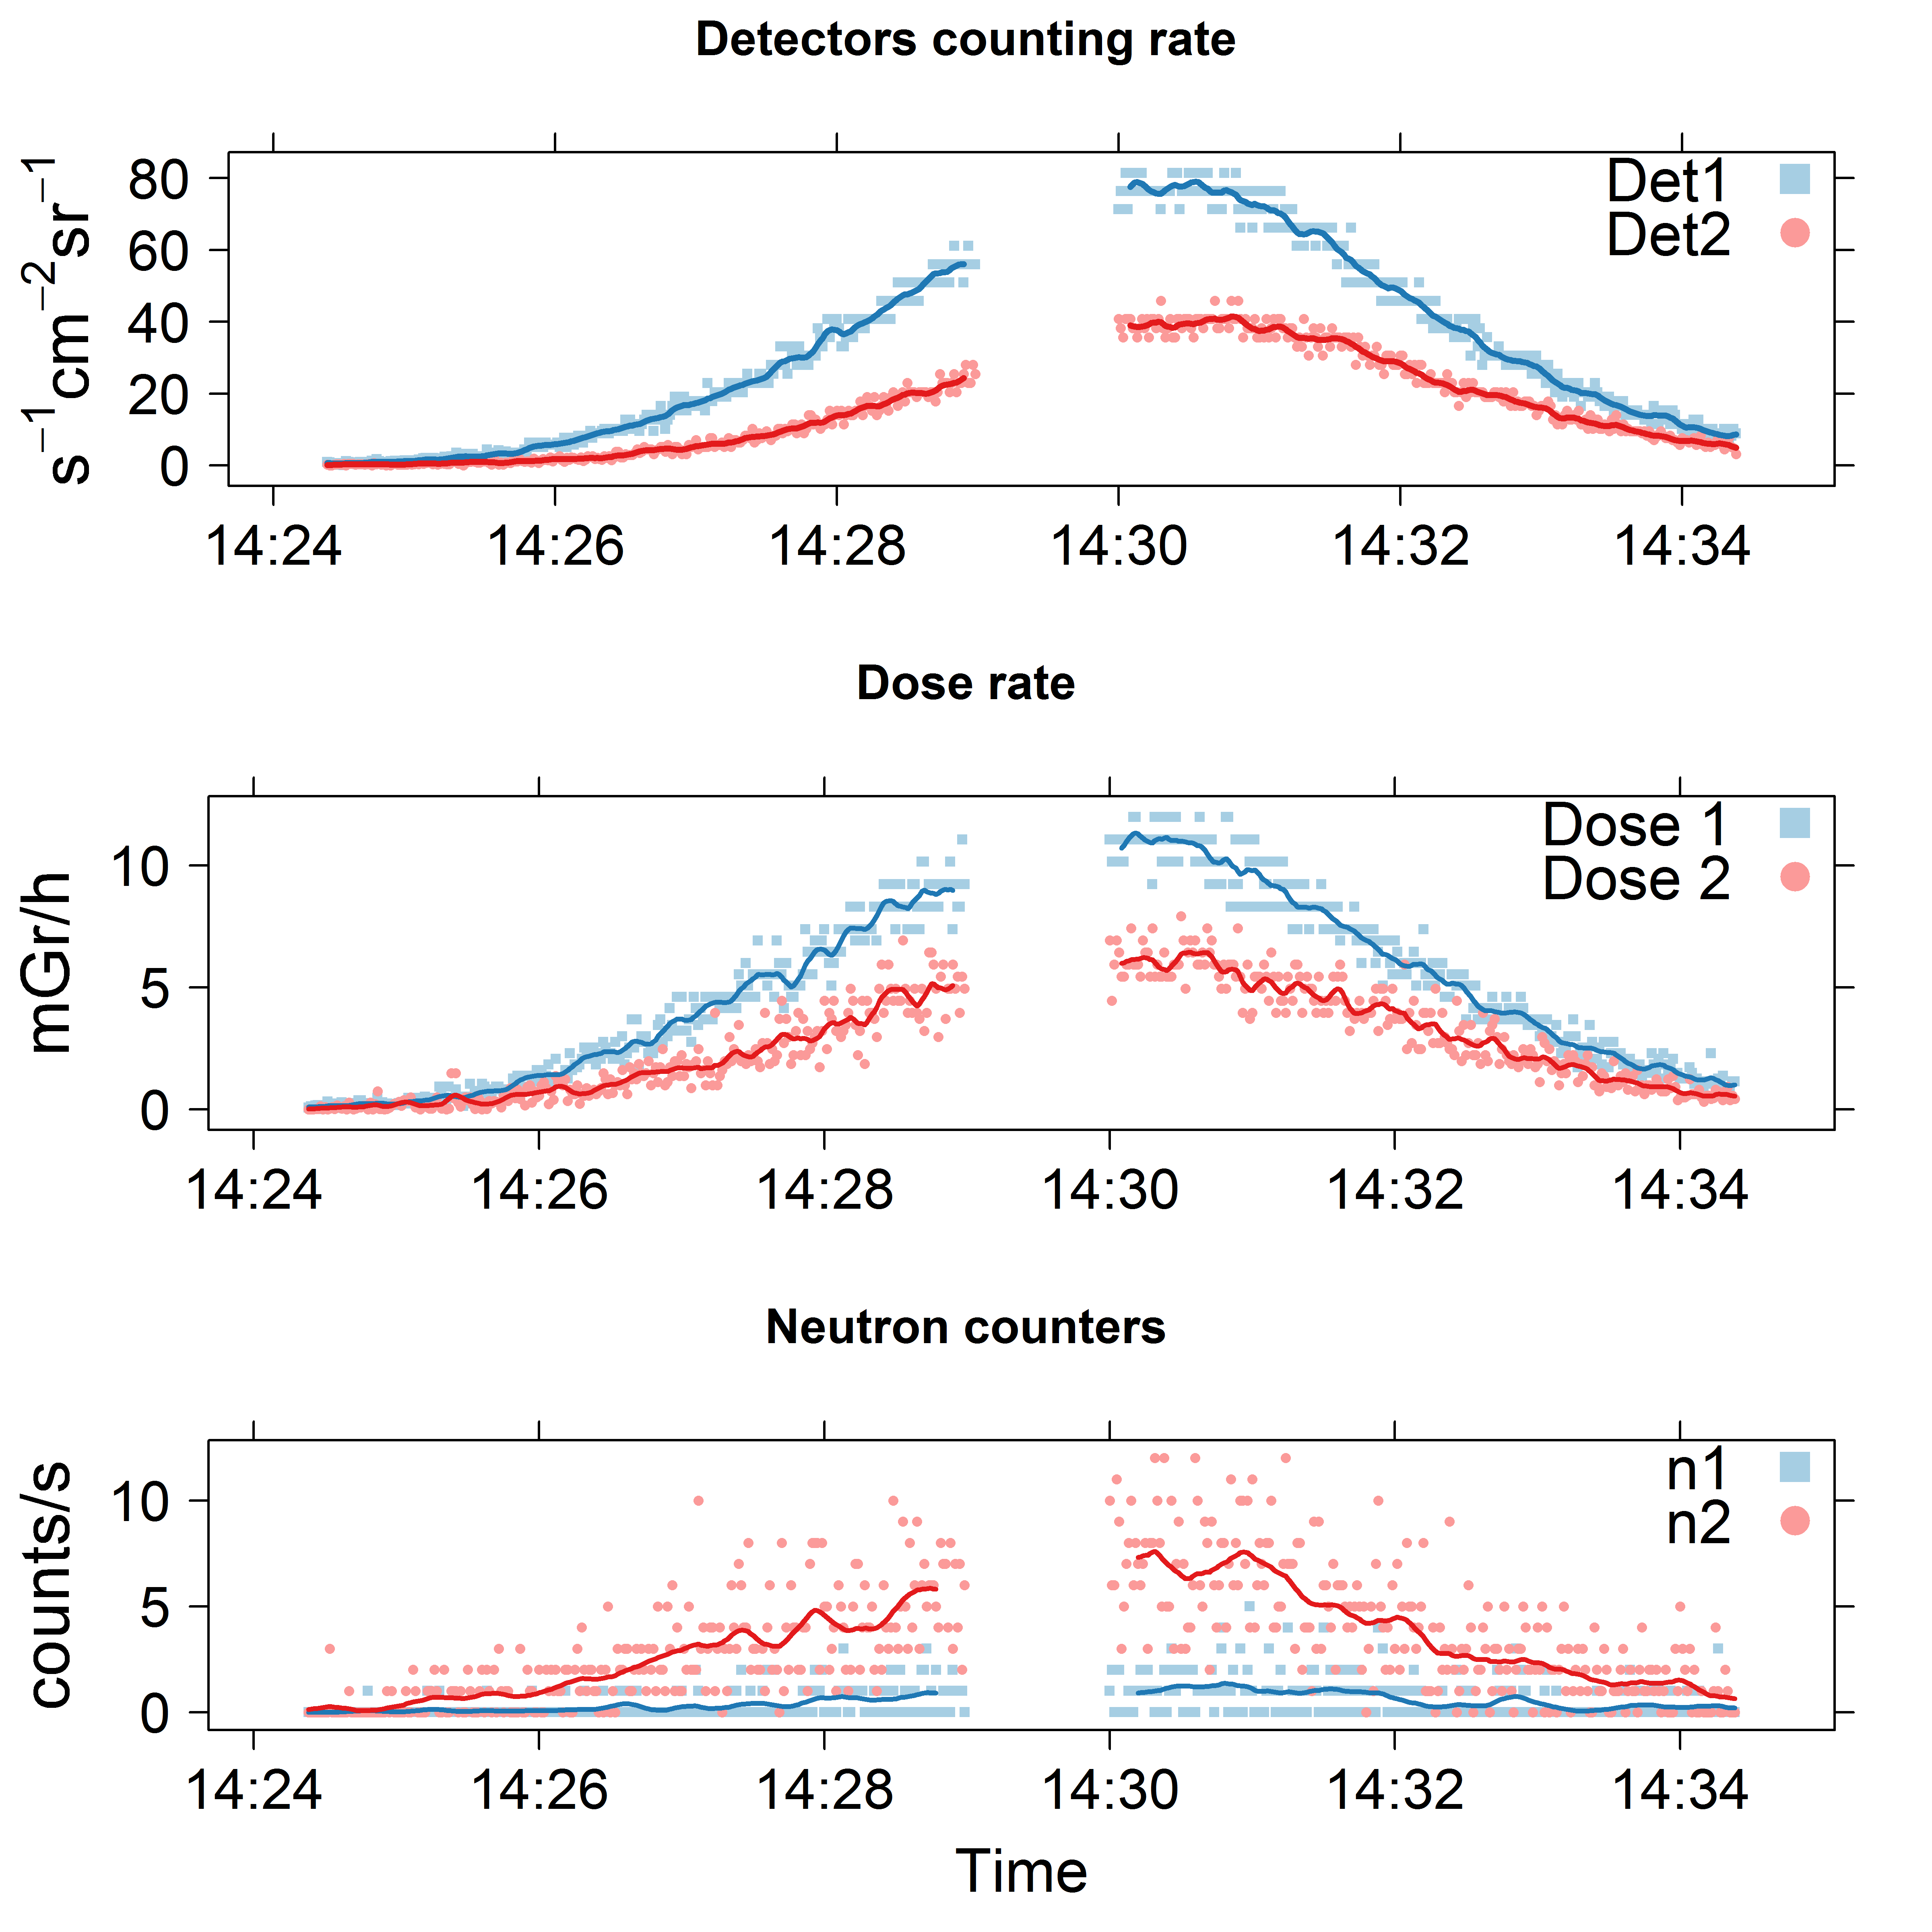
\includegraphics[width=0.5\linewidth]{images/results/depron_sec_log_new08-29-1614-24-23}
	\caption{Временные серии скоростей счета и мощности дозы при пересечении внутреннего радиационного пояса. }	\label{fig:depronseclognew08-29-1614-24-23}
\end{figure}

Видно, что в данных отсутствует минута измерений 14:29, это является последствием загруженности канала передачи данных. Также можно наблюдать, что верхний полупроводниковый детектор показывает потоки в два раза превышающие потоки во втором детекторе. Причем, важно отметить, что эти значения уже нормированы на геометрический фактор и представляют собой истинные интегральные потоки для заряженных частиц, различающиеся только нижней границей энергии регистрации. Подробнее границы энергетической чувствительности обсуждаются в разделе \ref{sec:energy}.

Аналогично потокам частиц, поглощенные дозы в аномалии относятся с фактором 2. Совпадение  величины отношения дозы и отношения счета частиц в двух детекторах показывает, что в зоне ЮАА половина частиц проникает через оба детектора и теряет незначительную долю энергии при прохождении через верхний детектор и разделяющие детекторы слои вещества в приборе. Те же частицы, которые не долетают до второго детектора имеют близкие энергетические характеристики, так как они вносят вклад в дозу прямо пропорциональный их потоку. Причиной такого характера работы полупроводниковых детекторов может являться более высокий порог регистрации у второго детектора по сравнению с первым детектором.

Счет в нейтронных счетчиках отличается более значительно, показания более защищенного детектора от 2 до 4 раз выше чем менее защищенного. Используя расчитанную относительную чувствительность нейтронных счетчиков \ref{fig:otnsensetiv},  можно предположить что максимум в спектре нейтронного излучения находится в диапазоне от 1 эВ до 1 КэВ.  Возможен также вариант того, что популяция зарегистрированных нейтронов является бимодальной по энергии. В таком случае мы не можем делать однозначные предположения о максимумах в энергетическом спектре потока нейтронов.

\begin{figure}
	\centering
	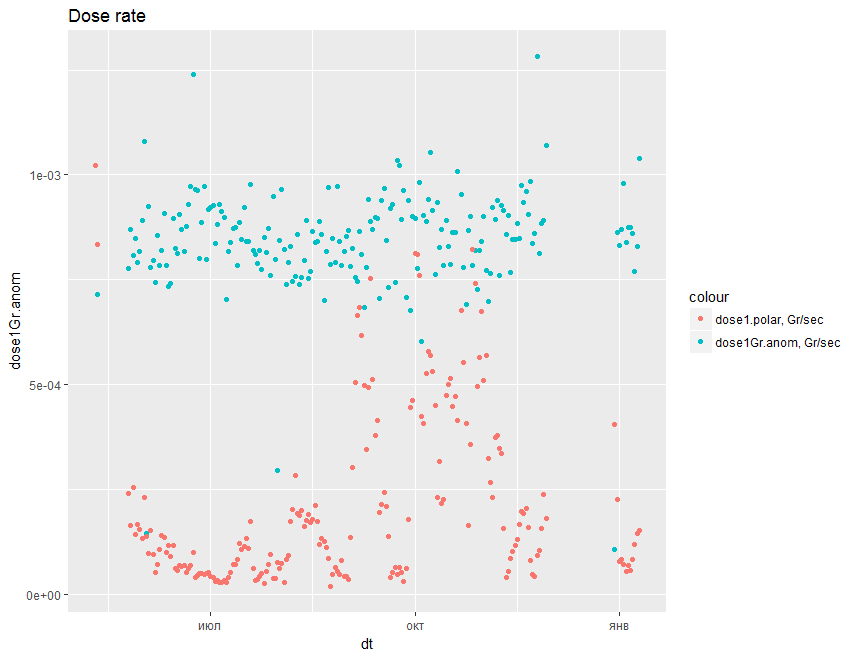
\includegraphics[width=0.49\linewidth]{images/doseanalisys/det1}
	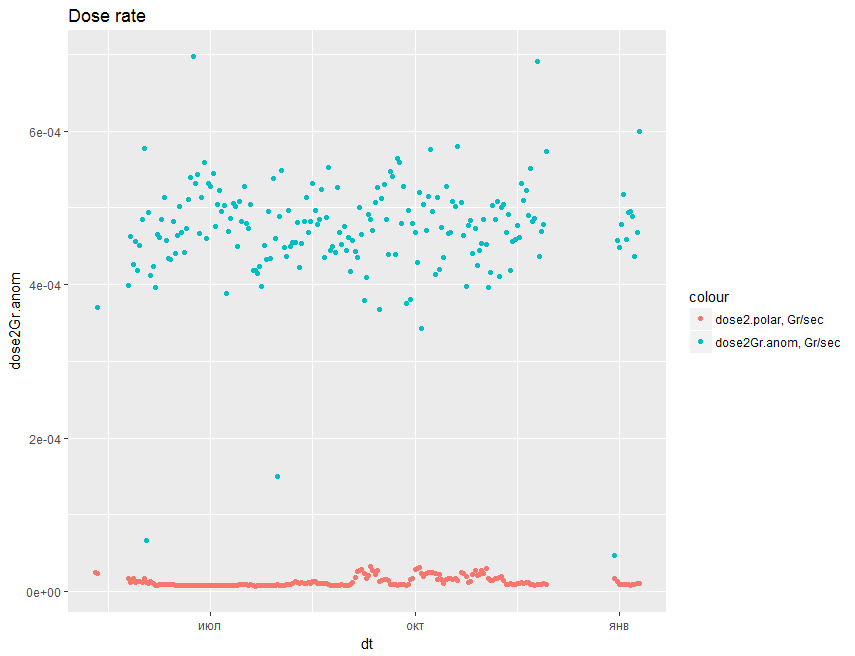
\includegraphics[width=0.49\linewidth]{images/doseanalisys/det2}
	\caption{ Левый график показывает среднесуточную мощность дозы в верхнем детекторе ДЭПРОН, правый график - в нижнем детекторе. Красные точки представляют среднесуточную мощность дозы в полярных регионах, зарегистрированную на спутнике Ломоносов. Синие точки - мощность дозы в моменты высокой скорости счета в аномалии.}
	\label{fig:doseanom}
\end{figure}

Средняя за день мощность дозы  представлена на рисунке \ref{fig:doseanom}. Для верхнего детектора она составляет около 7*10\textsuperscript{-4} Гр/с, при этом во втором детекторе мощность дозы меньше, чем в первом,  и составляет около 5*10\textsuperscript{-4} Гр/с. 

\section{Распределения мощности дозы в авроральных областях}

Мощность дозы в авроральных областях  в верхнем детекторе меняется за время проведения эксперимента в пределах от 10\textsuperscript{-4}  до 10\textsuperscript{-3} Гр/с  \ref{fig:doseanom}. Более защищенный детектор ДЭПРОН дает величины мощности дозы от  от 10\textsuperscript{-5}  до 10\textsuperscript{-3} Гр/с. Верхний детектор показывает возрастания поглощенной дозы на порядок величины во время повышения солнечной активности, эта связь более заметна для импульсных возрастаний потоков \ref{fig:rplot03}. Таким образом повышения потоков вносят заметный вклад в суточную дозу при пролетах высокоширотных областей.

Также построены зависимости скорости счета от времени и параметра L \ref{fig:l-t2016}а. Для сравнения представлены результаты измерений электронов с энергиями более 2 МэВ на спутниках Van Allen \ref{fig:l-t2016}б. 

\def\imagetop#1{\vtop{\null\hbox{#1}}}
\begin{figure}
%	\centering
	\begin{tabular}{l l}
		\imagetop{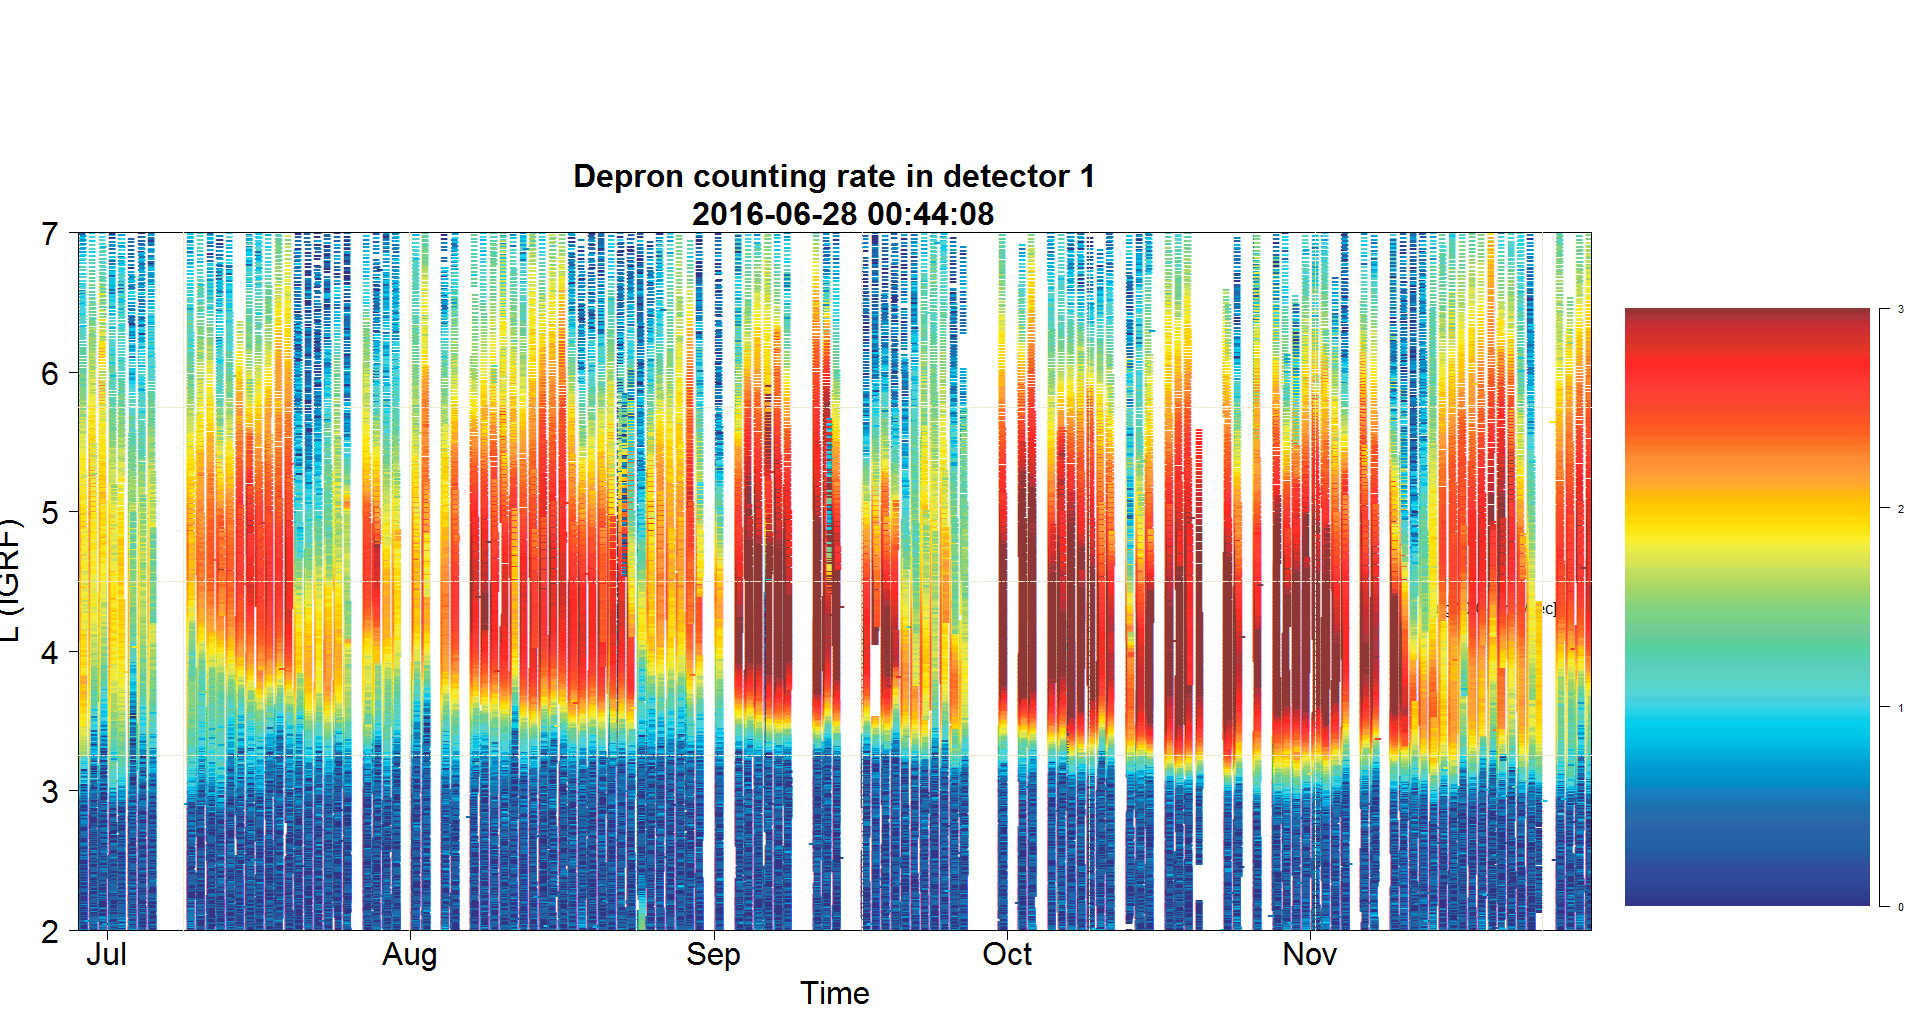
\includegraphics[width=0.9\linewidth, height = 0.2\textheight ]{images/L-t2016}} & \imagetop{(а)} \\
		\imagetop{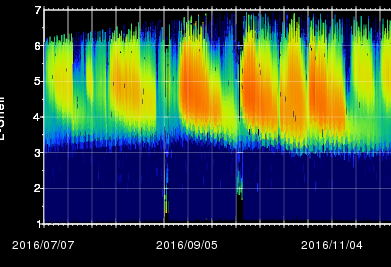
\includegraphics[width=0.75\linewidth, height = 0.16\textheight]{../literature_repository/relelec/van-allen-lshell-crop-sm}}& \imagetop{(б)}\\
		\imagetop{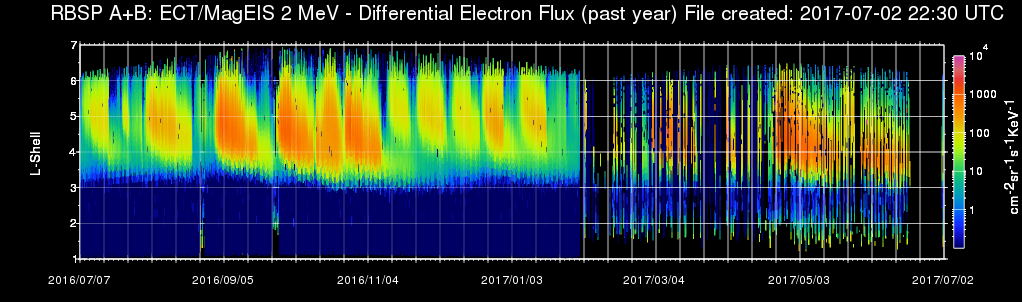
\includegraphics[width=0.9\linewidth]{../literature_repository/relelec/van-allen-lshell-crop-box}} & \imagetop{(в)}
	\end{tabular}
	\caption{а. Зависимость скорости счета в первом детекторе ДЭПРОН от времени и параметра Мак-Илвайна L.\\ б-в. Дифференциальный поток электронов с энергией более 2 МэВ, по данным спутников RPSB A и RPSB B.  По материалам: \cite{NOAA}. \\ Желтым прямоугольником выделен интервал времени, соответствующий времени проведения эксперимента ДЭПРОН. }
	
	\label{fig:l-t2016}
\end{figure}


\section{Анализ возрастаний потоков частиц в областях внешнего радиационного пояса}\label{sec:flash_analisys}
В  данных  ДЭПРОН приполярные области отличаются высокой вариабельностью во времени и пространстве потоков частиц и соответственно доз. Были найдены и выделены возрастания скоростей счета в первом детекторе	\label{fig:depronlatmap148}, превышающие по абсолютной величине 5000 отсчетов в секунду, что соответствует более 800 с\textsuperscript{-1} см\textsuperscript{-1} стер\textsuperscript{-1}. 
\begin{figure}[h]
	\centering
	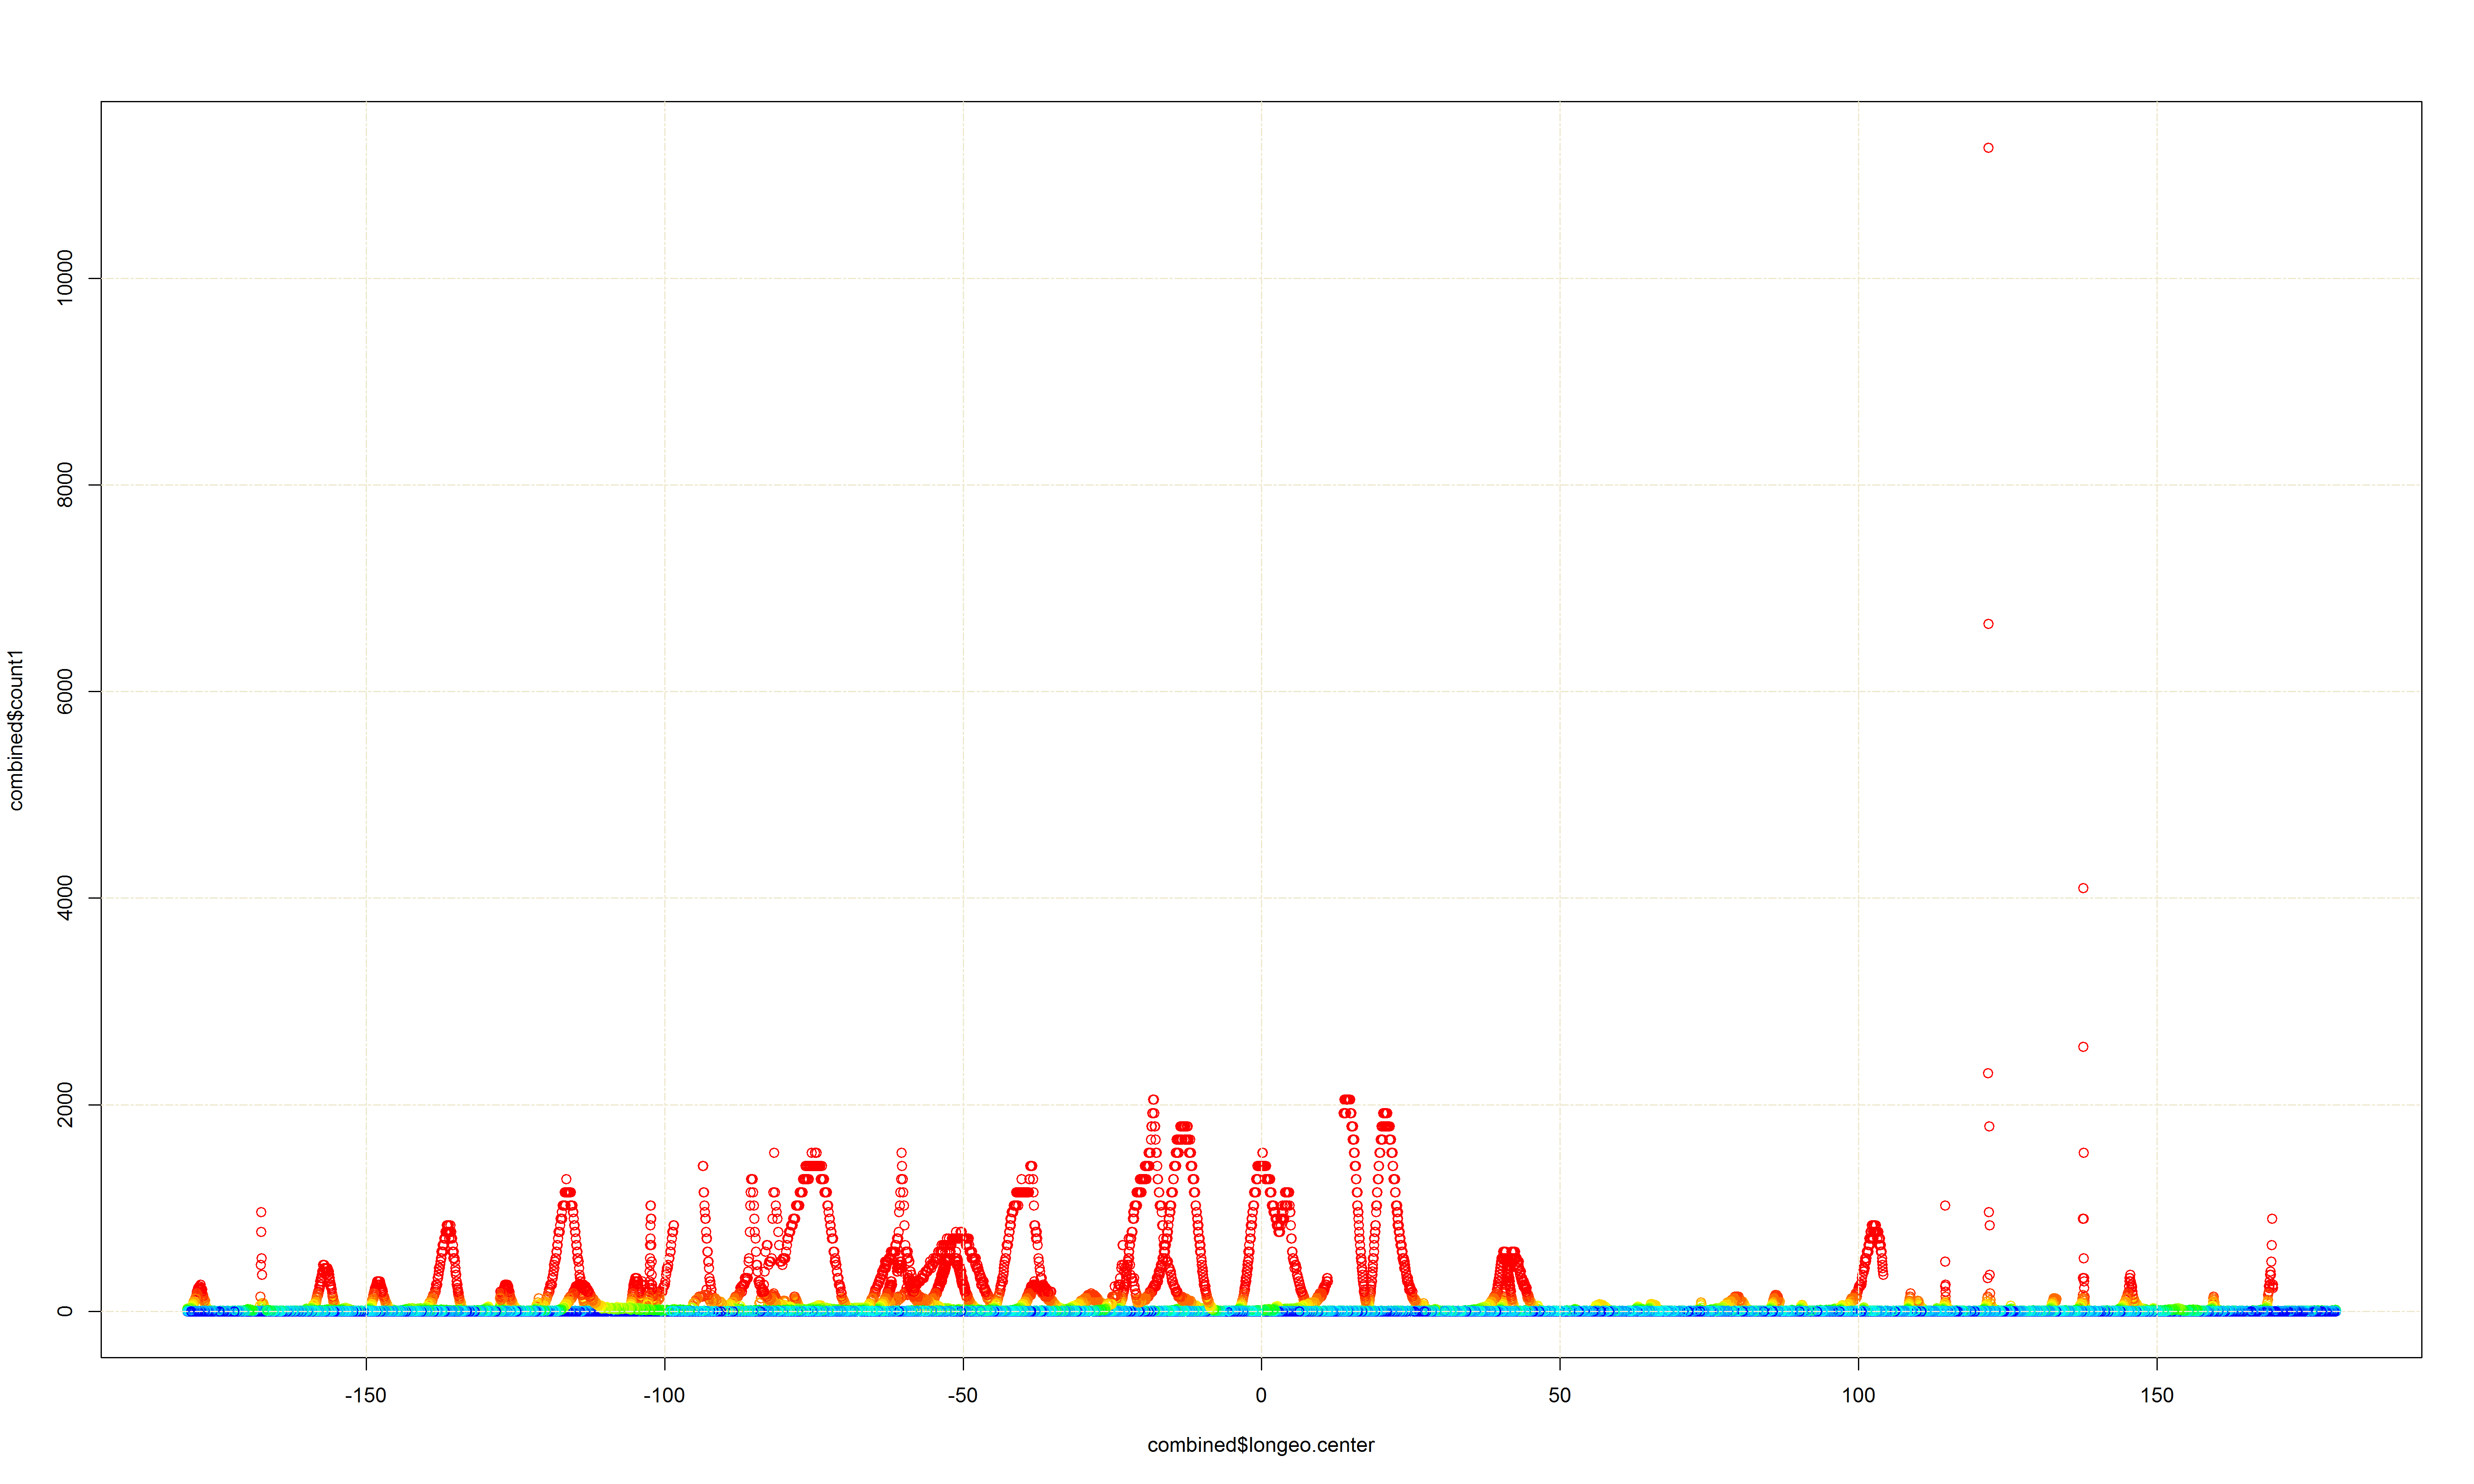
\includegraphics[width=0.8\linewidth]{images/Flash/depron_lat_map_148}
	\caption{Географическое распределение потоков заряженных частиц в первом полупроводниковом детекторе. Для наглядности счет в детекторе показан в линейном масштабе.}
	\label{fig:depronlatmap148}
\end{figure}
Величины повышенных потоков, зарегистрированных в первом полупроводниковом детекторе в среднем в 30-100 раз выше чем во втором детекторе и при одновременной регистрации в двух детекторах.
\begin{figure}[h]
	\centering
	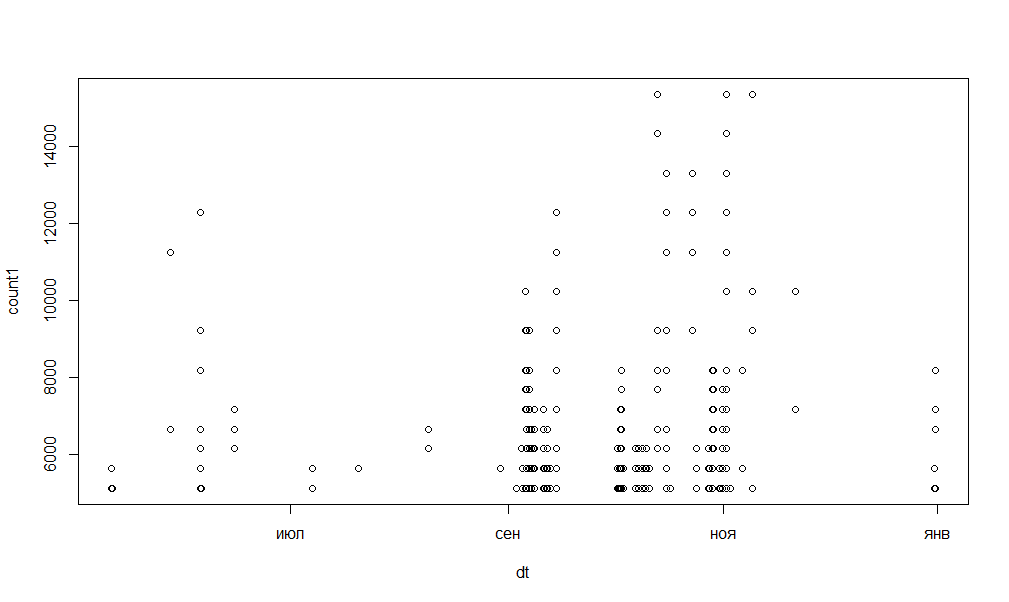
\includegraphics[width=0.7\linewidth, trim={0 2cm 0 0}]{images/Flash/Rplot03.png}
	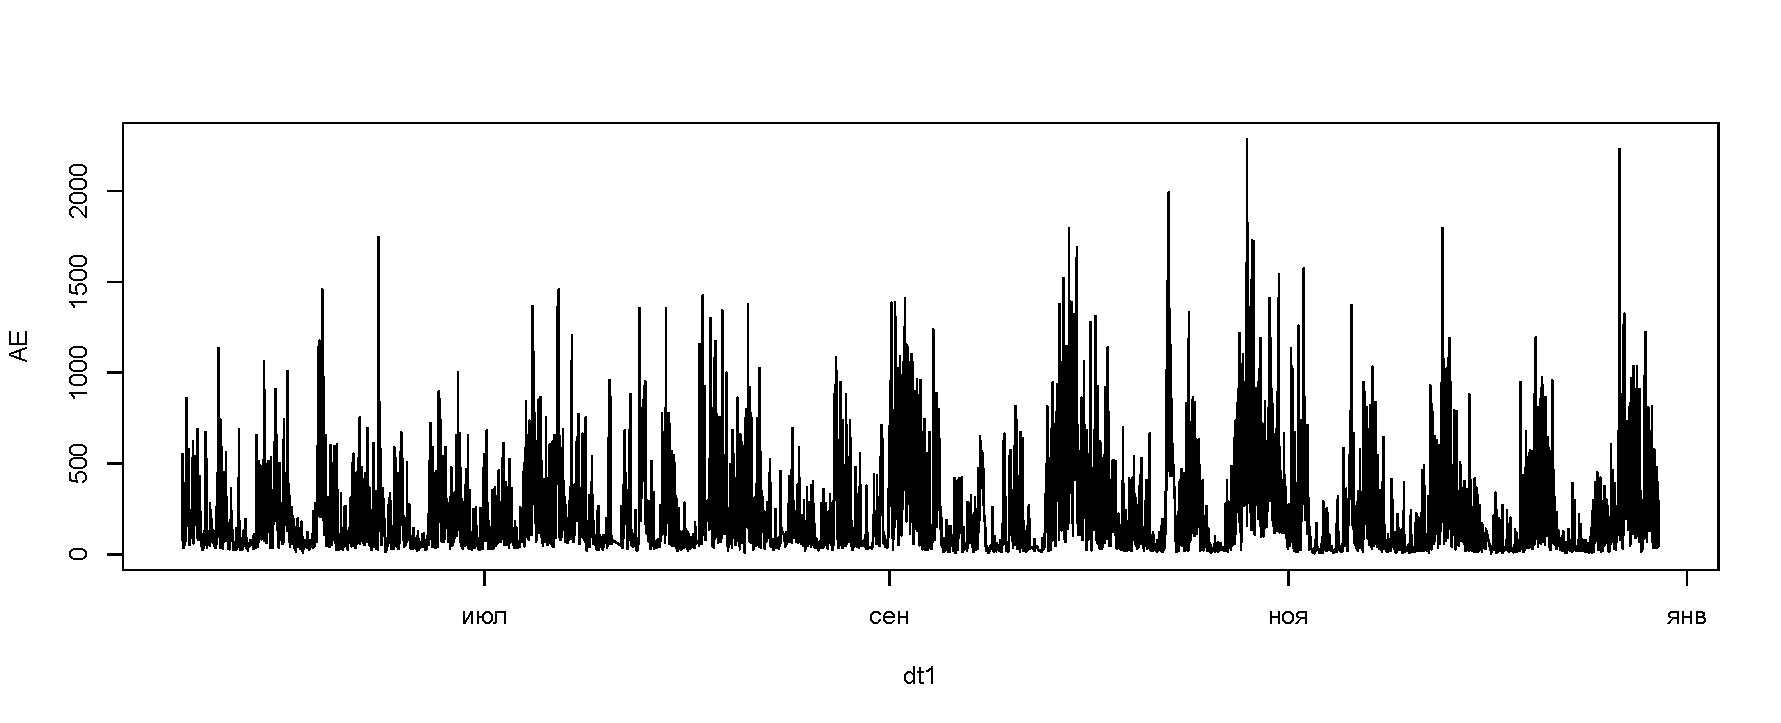
\includegraphics[width=0.7\linewidth, trim={0 1.5cm 0 0}]{images/Flash/Rplot01}
	\caption{Временное распределение зарегистрированных вспышек. Общее число выделенных вспышек за время работы прибора ДЭПРОН достигает 90. Второй график показывает вариации индекса AE, при отрицательном Bz. Данные предоставлены сервисом  \href{https://omniweb.gsfc.nasa.gov/}{OMNIweb}.}
	\label{fig:rplot03}
\end{figure}


Учитывая, что геометрический фактор телескопа детекторов в 3 раза меньше чем геометрический фактор верхнего детектора, мы можем предположить что энергии частиц в этих потоках невысоки, поэтому большая часть частиц до второго детектора не доходит.	Для наибольших возрастаний счета отношение скоростей счета меньше и составляет один порядок и здесь энергия частиц больше. Мы наблюдаем четкое разделение по скорости счета и соотношению в верхнем и нижнем детекторах. 
\begin{figure}[h]
	\centering
	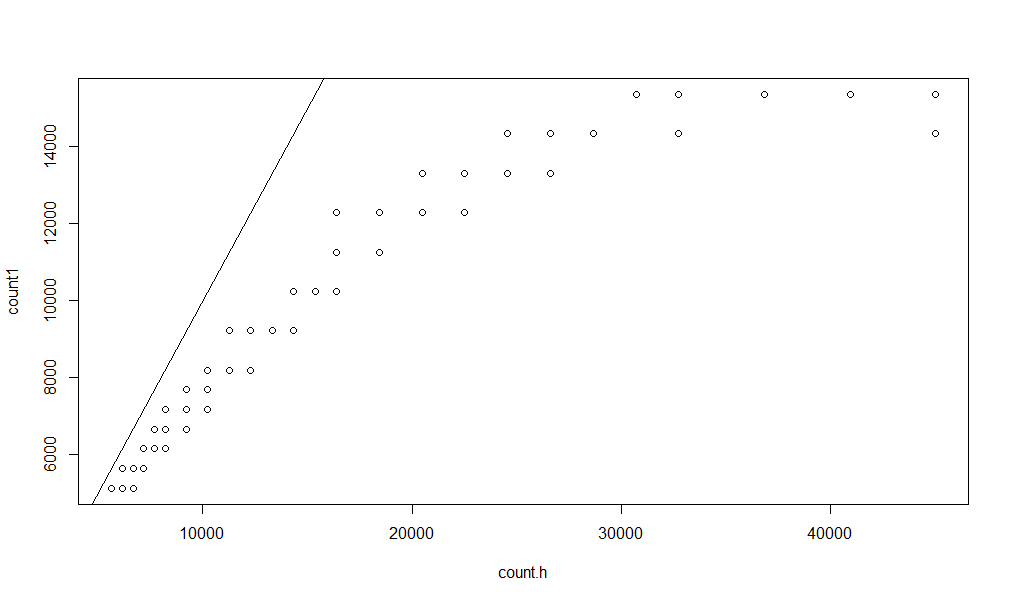
\includegraphics[width=0.7\linewidth]{images/Flash/Rplot04}
	\caption{Соотношение программного и аппаратного счетчиков для моментов времени, в которые регистрировались вспышки. Прямая на рисунке показывает соотношение, при котором все зарегистрированные частицы обработаны программой прибора. Каждая точка показывает интегральный счет за одну секунду.}
	\label{fig:rplot04}
\end{figure}
Соотношение аппаратного счетчика первого детектора и программного счетчика позволяет сделать вывод, что при высоких загрузках микроконтроллер ДЭПРОН не успевает программно обработать все зарегистрированные детекторами частицы. Зависимость \ref{fig:rplot04} отношения обработанных и всех частиц практически линейна до скоростей счета 5000 за секунду, а более 10 тысяч отсчетов становиться нелинейной. Поэтому в максимальных импульсах, зарегистрированных за время работы ДЭПРОН, не было обработано в три раза больше прерываний от частиц, по сравнению с числом обработанных программных прерываний. Это обстоятельство позволяет сделать поправки в большую сторону при оценке дозовых нагрузок во время вспышек. 

Для анализа различных параметров возрастаний были построены матричные графики всех доступных переменных друг относительно друга 	\ref{fig:rplot08}. Можно заметить, что параметр L меняется в пределах от 3 до 5,5. При этом максимальные величины потоков были зарегистрированы на L оболочке равной четырем. Значения напряженности магнитного поля B находятся в пределах от 0,26 до 0,5 Гн. Максимальные потоки были зарегистрированы при B около 0,35 Гн. 

Нейтронные счетчики в моменты регистрации вспышек не показывают какого-либо увеличения счета. Максимальные значения 2-3 отсчета в секунду, а средние величины менее 1 нейтронов за 5 секунд, они являются нормальными для данных широт. 

Для верного анализа вспышек, по мнению Е.Е. Антоновой, следует выбрать спокойный период солнечной активности, и о наличии магнитной бури судить по индексам A(e) и A(l) \ref{fig:rplot08}. 

Далее был проведен анализ наблюдений на периоды утреннего в вечернего местного магнитного врем (MLT). Следуя указаниям  Е.Е. Антоновой для всех вспышек был построен график распределения по MLT \ref{fig:rplot15}. На протяжении суток спутник несколько раз проходит по всем возможным MLT от 0 до 24 часов, в полярных зонах при этом, спутник находится при MLT либо 12 либо 24 часа. Но несмотря на это, можно заметить, что во время зарегистрированных вспышек, MLT,  в основном, принимает значение от 21 до 23 часов. Также есть несколько измерений, для которых MLT принимает значение 0 и около 12 часов. На основе этих графиков можно сделать вывод о несоответствии ожидаемой частоты наблюдаемого MLT и той, что характерна для вспышек. Вспышки наблюдаются в основном с 21 час и по мере приближения к полночи их число уменьшается.


\begin{figure}
	\centering
	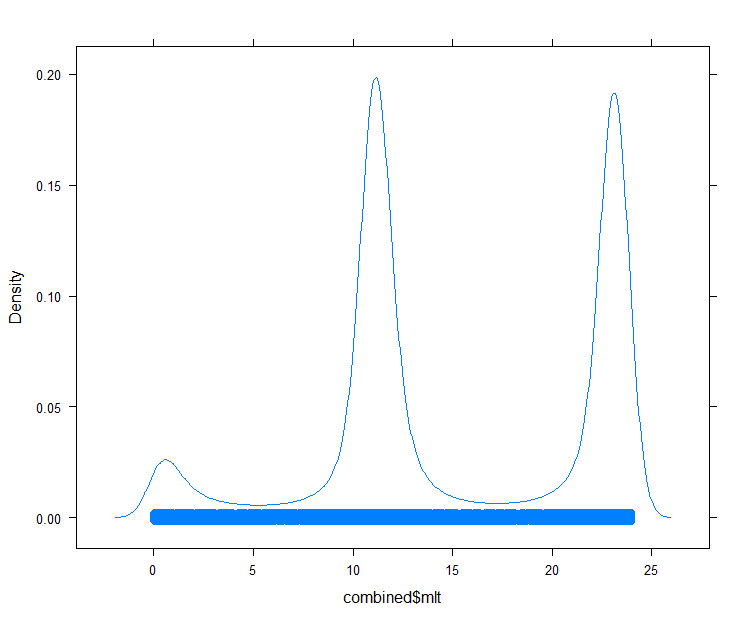
\includegraphics[width=0.49\linewidth]{images/Flash/Rplot020}
	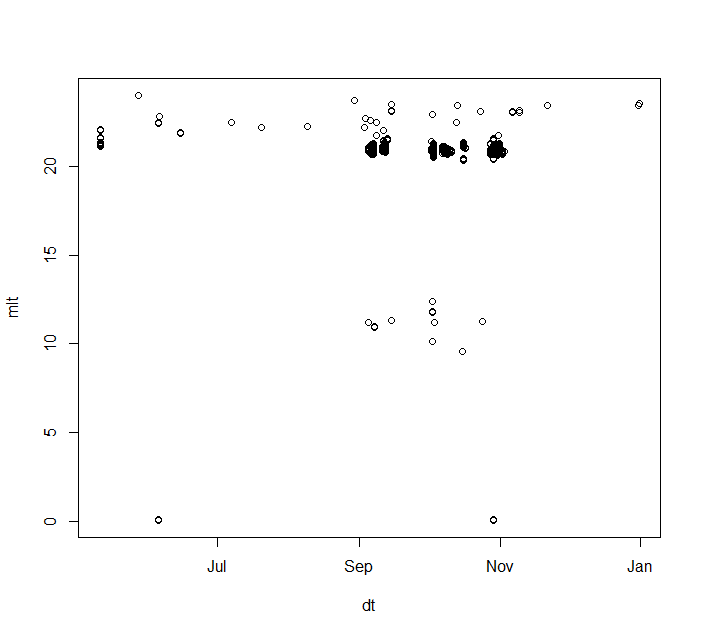
\includegraphics[width=0.49\linewidth]{images/Flash/Rplot14}
	\caption{Слева: Плотность вероятности наблюдения различных значений магнитного локального времени в точках с координатами пролета спутника Ломоносов за период времени в одни сутки для полярных областей. \\Справа: Магнитное локальное время для зарегистрированных за все время вспышек.}
	\label{fig:rplot15}
\end{figure}


\begin{figure}
	\centering
	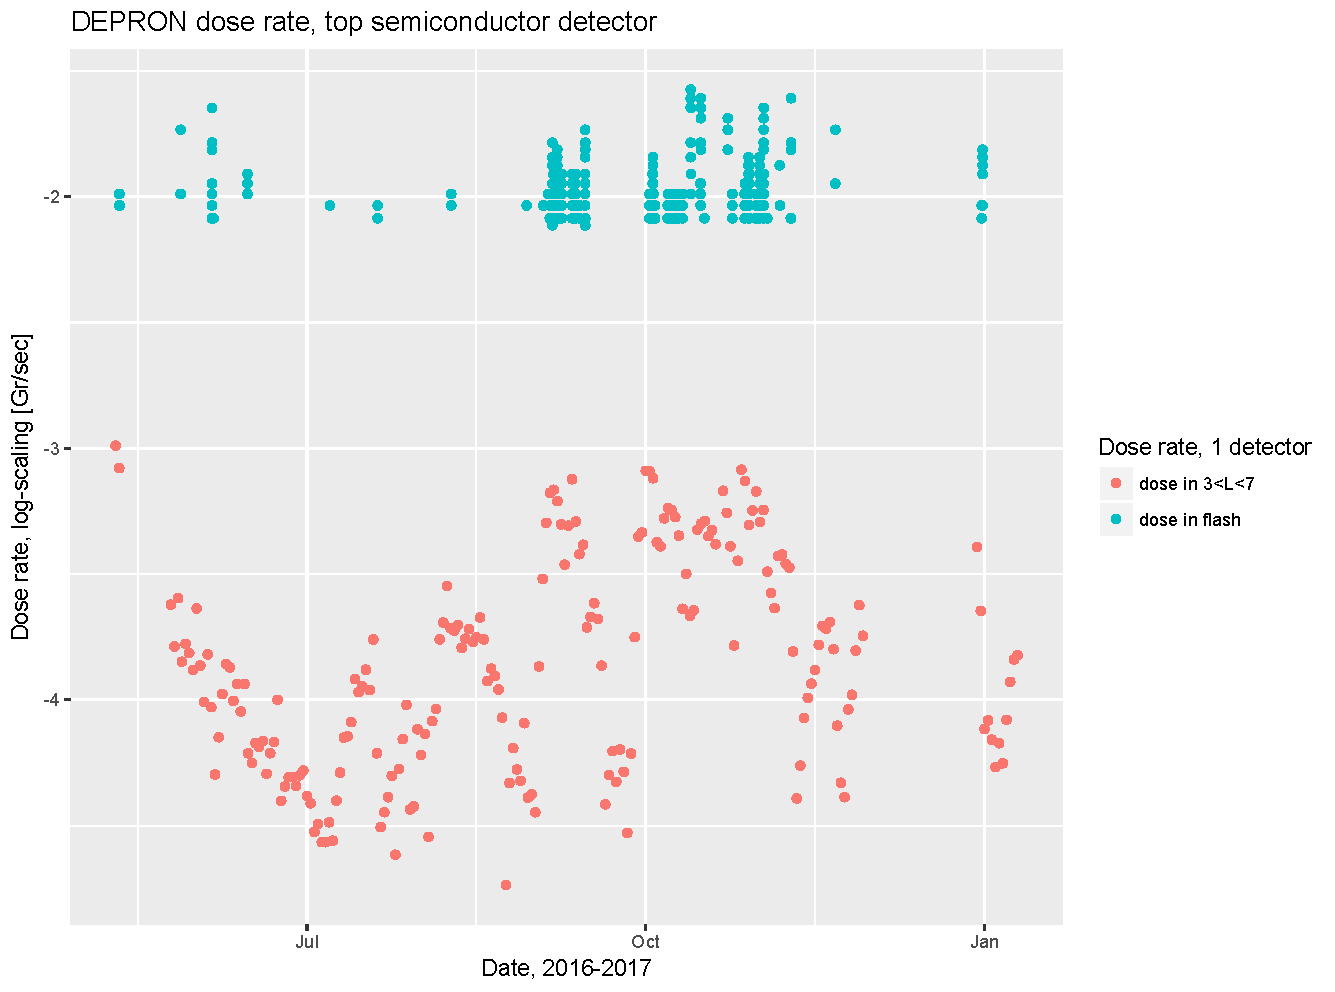
\includegraphics[width=0.49\linewidth]{images/doseanalisys/flashdose1}
	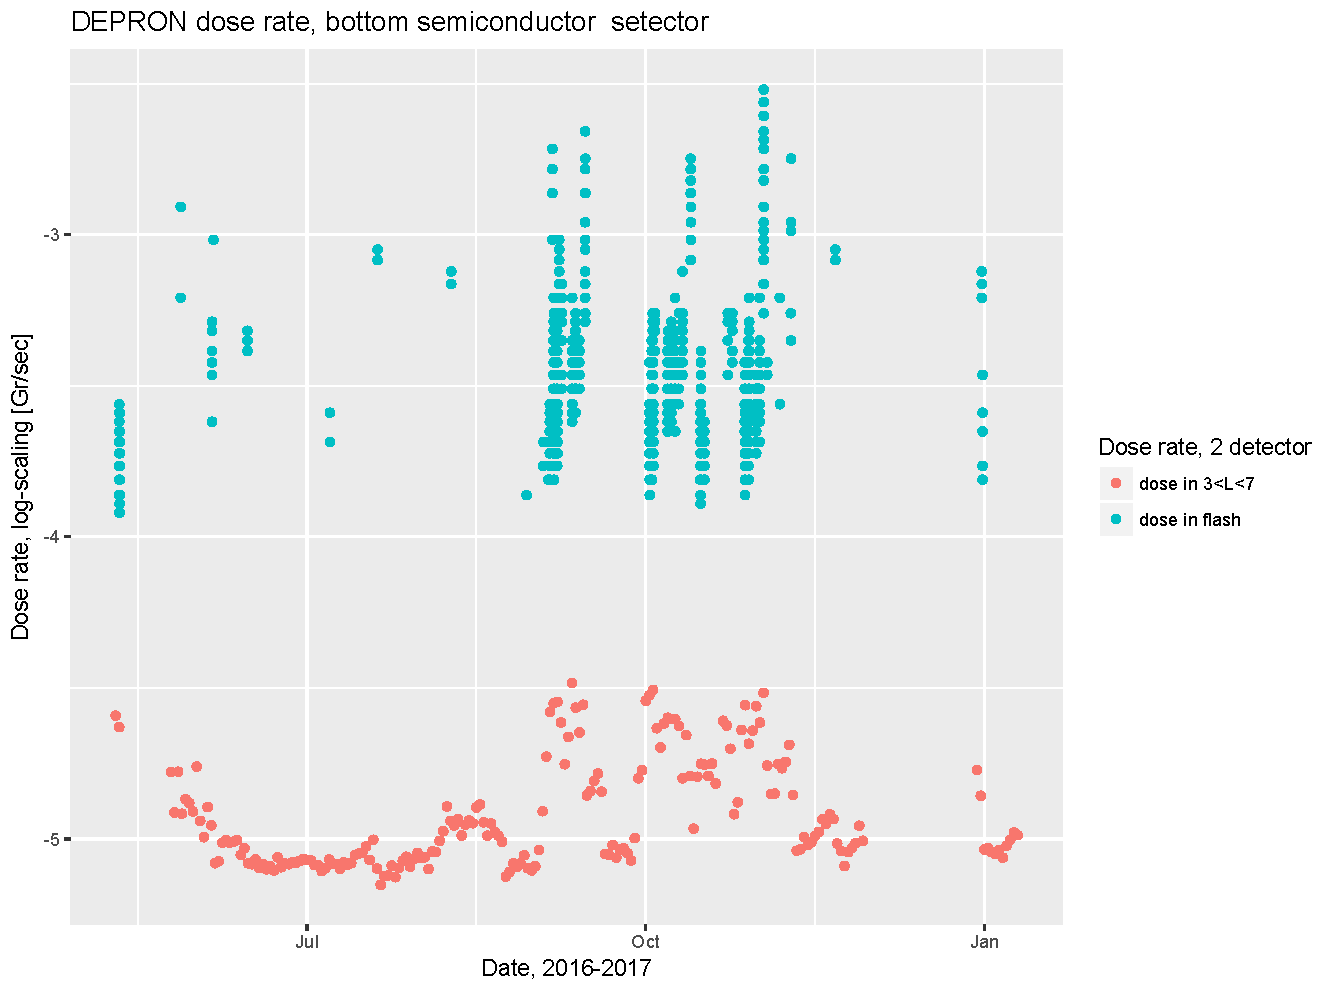
\includegraphics[width=0.49\linewidth]{images/doseanalisys/flashdose2}
	\caption{Красные точки показывают среднесуточную мощность дозы в полярных регионах, зарегистрированных на спутнике Ломоносов. Синие точки - мощность дозы в моменты высокой скорости счета в верхнем детекторе DEPRON.}
	\label{fig:flashdose1}
\end{figure}
Мы можем считать, что короткие вспышки вносят существенный вклад в  суммарную дозу в обоих детекторах. Этот вклад более значителен в полярных областях и достигает одного порядка величины для верхнего детектора и половину порядка для нижнего детектора по поглощенной дозе \ref{fig:flashdose1}. Для вспышки, зарегистрированной в 2016-10-28 21:43:42 --- 21:45:26UTC поглощенная доза для верхнего детектора превышает 1 Гр. Данная вспышка отличается наибольшей по сравнению с другими вспышками продолжительностью - 105 секунд \ref{fig:rplot12}.

\begin{figure}
	\centering
	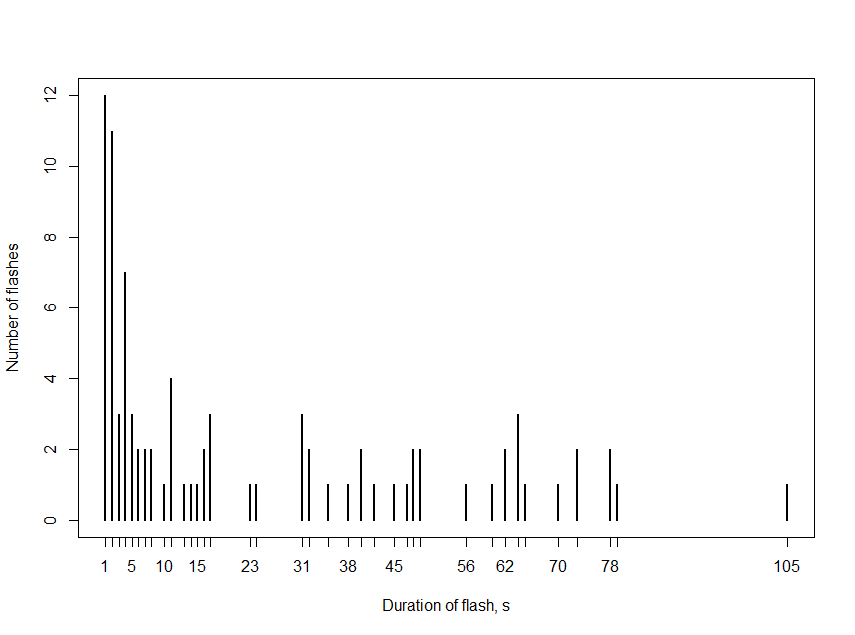
\includegraphics[width=0.7\linewidth]{images/Flash/Rplot12}
	\caption{Распределение наблюдаемых вспышек по длительности. Две трети вспышек имеют длительность менее 20 секунд.}
	\label{fig:rplot12}
\end{figure}




\begin{figure}
	\centering
	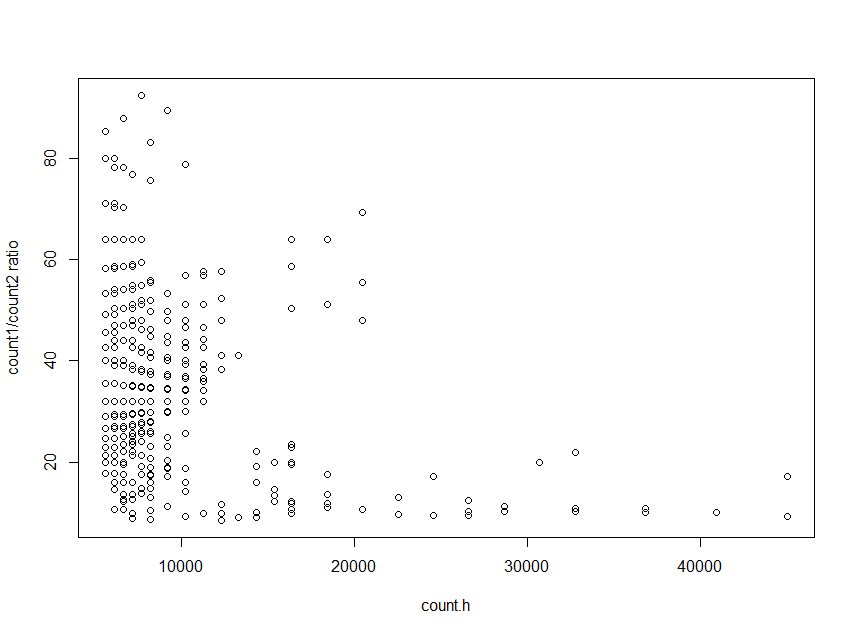
\includegraphics[width=0.7\linewidth]{images/Flash/Rplot11}
	\caption{Соотношение скоростей счета в детекторах. По оси абсцисс отложен счет в Данная зависимость позволяет разделить возрастания по жесткости и мощности на две группы.}
	\label{fig:rplot11}
\end{figure}

При подробном рассмотрении соотношения поглощенных доз в детекторах ДЭПРОН во время вспышек \ref{fig:rplot03}, большинство возрастаний проявляют линейную зависимость дозы в верхнем детекторе по отношению к дозе в нижнем детекторе.
\begin{figure}
	\centering
	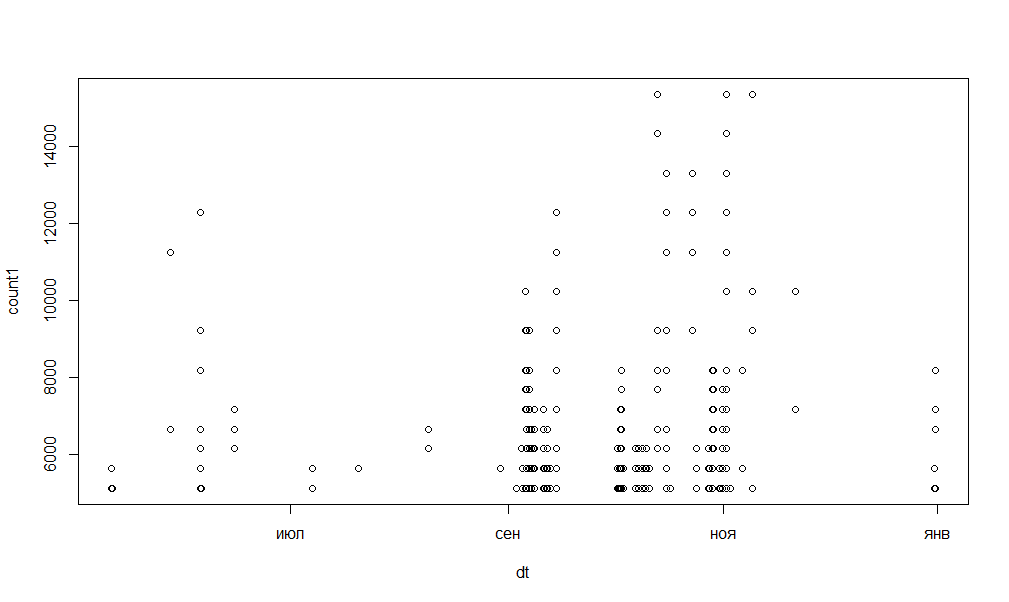
\includegraphics[width=0.7\linewidth]{images/Flash/Rplot03}
	\caption{Распределение вспышек по величине интегральных поглощенных доз за каждое возрастания. По оси абсцисс отложены поглощенные дозы в верхнем детекторе, а по оси ординат величины доз во втором, более глубоком детекторе.}
	\label{fig:rplot03}
\end{figure} 
Выделяется только событие второго Ноября 2016 в 00:42 UTC, во время этого события доза во втором детекторе в 4 раза превышает величину, соответствующую линейной пропорциональности доз в детекторах. Величина дозы за это событие составляет 0,08 Гр, что является абсолютным максимум поглощенной дозы во втором детекторе за все время эксперимента. Длительность события 2016-11-02 составляет 40 секунд. Детально рассмотреть это событие можно используя график 	\ref{fig:depronseclognew11-02-16}. Форма пика во время события двойная, сначала скорость счета и доза в первом детекторе выходит на уровень около 800 частиц/c*см\textsuperscript{2}*ср, затем за минуту она достигает максимума в 2,5 тысячи частиц/c*см\textsuperscript{2}*ср и спадает опять до величины 800 частиц/c*см\textsuperscript{2}*ср. Дозу за секунду во втором детекторе показывают красные точки на правом графике \ref{fig:depronseclognew11-02-16}, дозу в первом детекторе показывают синие точки. График потоков для второго детектора содержит особенности, отсутствующие на графике для верхнего детектора - небольшие возрастания при входе в зону. У данной особенности может быть два объяснения: первое --- это то, что на внешней границе радиационных поясов потоки зараженных частиц выше, а второе --- то, что электроника прибора не справляется с обработкой растущих потоков и во втором детекторе наблюдаются просчеты. 
Такой выброс поглощенной дозы во втором детекторе может соответствовать потоку частиц, обладающих высокой проникающей способностью.
\begin{figure}
	\centering
	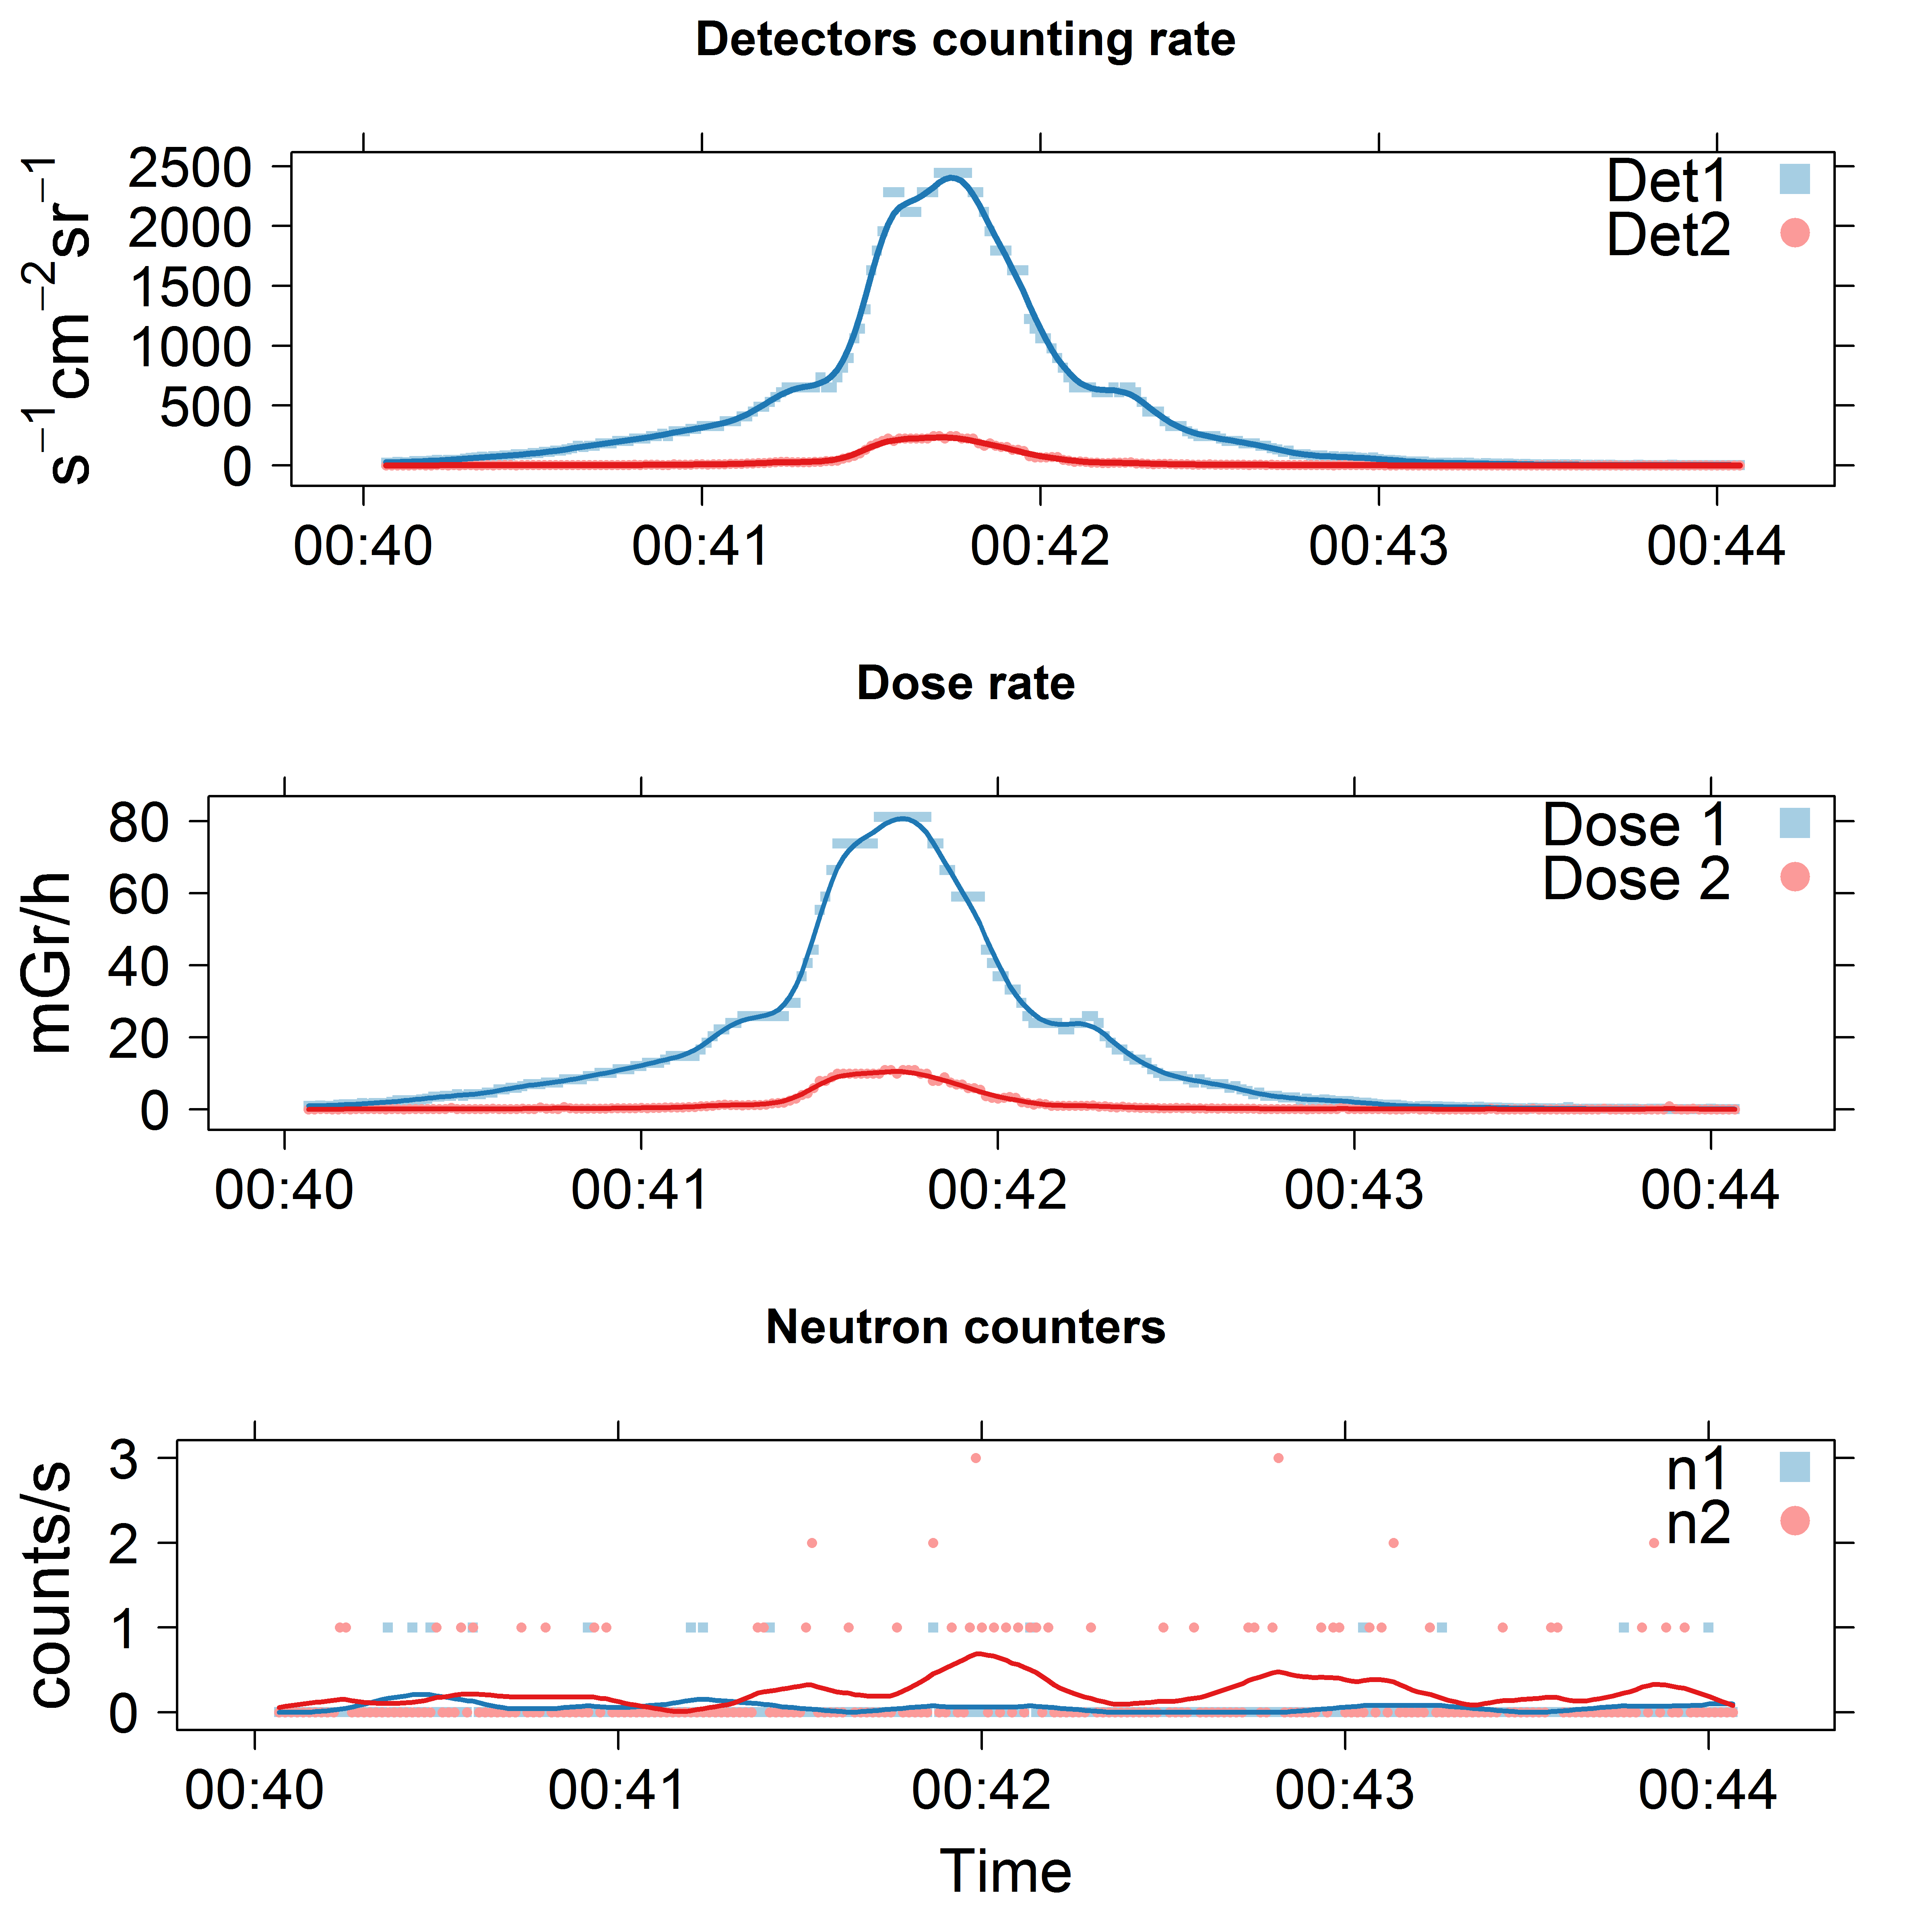
\includegraphics[width=0.49\linewidth]{images/Flash/depron_sec_log_new11-02-16}
	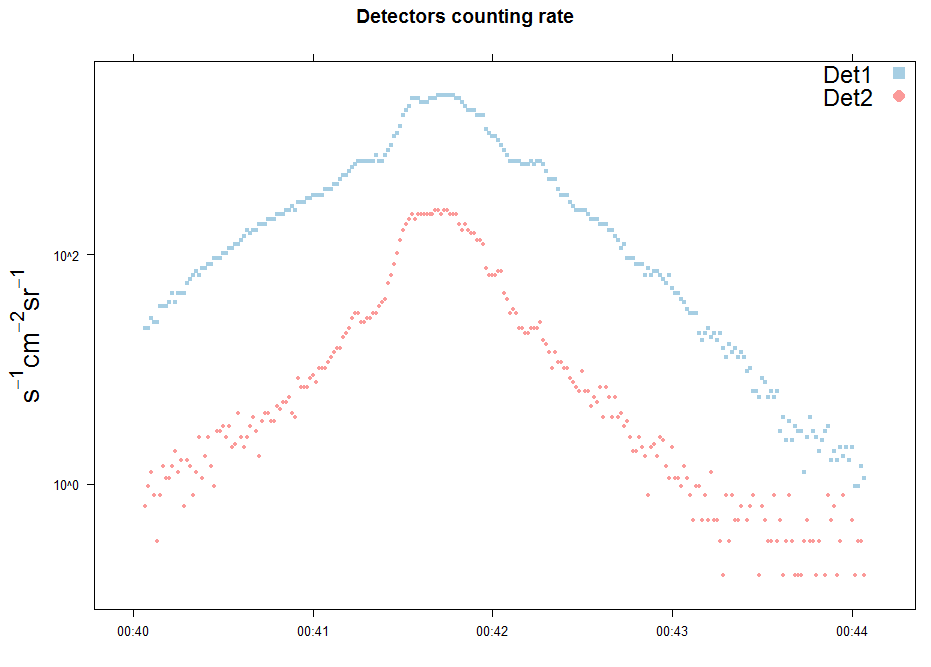
\includegraphics[width=0.49\linewidth]{images/Flash/depron_sec_log_new11-02-161}
	\caption{Временной профиль возрастания, зарегистрированный 2 Ноября 2016 года в 00:40 по мировому времени.}
	\label{fig:depronseclognew11-02-16}
\end{figure}



%Были рассмотрены зависимости дозы в L-B координатах.
%Построены зависимости B(t) для L из диапазонов от 4-5, 5-6, 6-7.


%\section{Спектры ЛПЭ и распределение мощности эквивалентной дозы}